% ============================================================================
%  Epilepsy Temple: a complete research record
%  Compile from this folder with:  latexmk -pdf main.tex   (or pdflatex x2)
% ============================================================================
\documentclass[11pt,a4paper]{article}

\usepackage[utf8]{inputenc}
\usepackage[T1]{fontenc}
\usepackage{lmodern}
\usepackage{textcomp}
\usepackage[margin=2.2cm]{geometry}
\usepackage{amsmath,amssymb}
\usepackage{graphicx}
\usepackage{booktabs}
\usepackage{tabularx}
\usepackage{longtable}
\usepackage{array}
\usepackage{float}
\usepackage{caption}
\usepackage{xcolor}
\usepackage{enumitem}
\usepackage{microtype}
\usepackage[hidelinks]{hyperref}

\setlength{\parskip}{4pt}
\setlist{itemsep=1pt,topsep=3pt}
\captionsetup{font=small,labelfont=bf}
\renewcommand{\arraystretch}{1.15}
\newcolumntype{L}{>{\raggedright\arraybackslash}X}
\graphicspath{{../}}

% --- ions and units (text mode) ---
\newcommand{\Kp}{K\textsuperscript{+}}
\newcommand{\Nap}{Na\textsuperscript{+}}
\newcommand{\Clm}{Cl\textsuperscript{$-$}}
\newcommand{\Catwo}{Ca\textsuperscript{2+}}
\newcommand{\HCO}{HCO\textsubscript{3}\textsuperscript{$-$}}
\newcommand{\Ko}{$[\mathrm{K}^+]_o$}
\newcommand{\Nai}{$[\mathrm{Na}^+]_i$}
\newcommand{\Cli}{$[\mathrm{Cl}^-]_i$}
\newcommand{\EGABA}{$E_{\mathrm{GABA}}$}
\newcommand{\uV}{\textmu V}
\newcommand{\us}{\textmu s}
\newcommand{\uM}{\textmu M}
\newcommand{\FAd}{FA/day}
\newcommand{\code}[1]{\texttt{\detokenize{#1}}}
\newcommand{\best}[1]{\textbf{#1}}

\title{\textbf{Epilepsy Temple}\\[4pt]
\large From a temple-worn optical wearable to a multimodal ``?''-shaped ear-hook seizure monitor:\\
research, biophysical simulation, inference, and detection on real patient data\\[6pt]
\normalsize A complete research record}
\author{Rhydham Mittal\\\small with Claude (Anthropic) as research and engineering assistant}
\date{29 September 2026}

\begin{document}
\maketitle

\begin{abstract}
\noindent
This paper records every step of a research project that asked whether a small consumer-style wearable could detect epileptic seizures. The starting point was \emph{Temple}, a temple-worn multi-wavelength photoplethysmography (PPG) device; a technical teardown showed that it measures scalp blood flow and cannot see the brain's electrical activity. We therefore (i)~reviewed epilepsy, the second-by-second neurophysiology of seizures and the whole-body physiological changes that accompany them; (ii)~built three seizure simulators of increasing realism, culminating in a 100-neuron conductance-based network with potassium, sodium, chloride, adenosine and haemodynamic dynamics that is validated against Cressman et al.\ (2009) and reproduces the ictal \Kp{} ceiling ($\approx$12\,mM), chloride loading, depolarising GABA, an adenosine surge, postictal silence, a \Kp{} undershoot and postictal hypoperfusion; (iii)~derived, audited and corrected the formulas needed to \emph{infer} hidden variables (\Kp, \Clm, $E_{\mathrm{GABA}}$, adenosine, excitation/inhibition balance, haemoglobin) from non-invasive signals, and tested them in twin experiments; (iv)~cross-validated our Epileptor against The Virtual Brain (identical first onset, 886.2); (v)~measured seizure detection on real scalp EEG (CHB-MIT, 23 subjects, 185 seizures), showing that two ear-level electrodes catch as many seizures as an 18-channel cap (88\% vs 85\% for a never-seen user) but with about twice the false alarms; (vi)~redesigned the concept as a bilateral ``?''-shaped ear-hook; (vii)~built an offline, single-screen interactive visualisation of the whole system; and (viii)~ran a large multimodal study on SeizeIT2 (125 patients, 883 seizures, 11,626\,h of behind-the-ear EEG, ECG, EMG and motion), streamed from the cloud through memory. Adding ECG to behind-the-ear EEG cut false alarms by 18--31\% at matched sensitivity and helped 115/125 patients; minute-scale context and a novel ``heart rate not explained by movement'' feature reduced false alarms by up to 62\% versus ear EEG alone; personal fine-tuning and a personal alarm verifier raised the share of seizures caught at $\le$1 false alarm/day from 4\% (ear EEG) to 19\% overall and to 39--40\% in ``heart responders''. All focal-to-bilateral tonic-clonic seizures were caught at $\le$5 false alarms/day, and simulated in-ear PPG retained most of the ECG benefit. A ceiling analysis showed that a quarter of seizures never raise the detector above 0.5: the remaining gap is a signal (hardware) problem, not an alarm-logic problem. Every experiment, result, failure, bug and correction is reported.
\end{abstract}

\noindent\textbf{Keywords:} epilepsy; wearable seizure detection; ear-EEG; behind-the-ear EEG; ECG; photoplethysmography; ion-concentration dynamics; Cressman model; Epileptor; The Virtual Brain; Bayesian inference; CHB-MIT; SeizeIT2; personalisation; false alarms.

\vspace{4pt}
\noindent\fbox{\parbox{0.97\linewidth}{\small\textbf{Disclaimer.} This is a research and educational project. Nothing here is a medical device or has been clinically validated; it must not be used to diagnose, monitor or treat epilepsy. Temple is a product of Temple Wearables / Continue Research; this project is independent and not affiliated with it.}}

\tableofcontents
\clearpage

% ============================================================================
\section{Introduction}
\label{sec:intro}

\subsection{Motivation}

About 50 million people live with epilepsy. Roughly one in three has drug-resistant seizures, and people with frequent tonic-clonic seizures carry a markedly raised risk of sudden unexpected death in epilepsy (SUDEP) that is reduced by nocturnal supervision and seizure alarms (Section~\ref{sec:background}). Patients also under-report their own seizures, so objective seizure counts are clinically valuable even when no alarm is raised. Existing cleared wearables (wrist accelerometry and electrodermal activity, upper-arm PPG, surface EMG) work well for \emph{convulsive} seizures but largely miss focal seizures, which are the majority.

In 2025--2026, Deepinder Goyal (founder of Zomato) presented \emph{Temple}, a small temple-worn optical wearable. This project began by asking what exactly Temple measures and whether a device of that size and at that location could detect seizures. The answer led, step by step, to a different device concept, a ``?''-shaped ear-hook worn on both ears that combines ear-EEG, in-ear PPG and motion sensing, and to a sequence of simulations and data studies to test it.

\subsection{Research questions}

The project was organised around a chain of questions, each answered by a document, a piece of code or an experiment (Table~\ref{tab:journey}).

\begin{table}[H]
\centering\small
\caption{Research journey: questions, methods and outputs.}
\label{tab:journey}
\begin{tabularx}{\linewidth}{@{}c L L@{}}
\toprule
\# & Question & Output (section) \\
\midrule
1 & What exactly is Temple, technically? & Technical dossier (\S\ref{sec:temple}) \\
2 & What is epilepsy, and what happens in the brain during a seizure? & Background review (\S\ref{sec:background}) \\
3 & Can seizures be simulated realistically, including ion concentrations? & Three simulators; ionic model validated against Cressman 2009 (\S\ref{sec:sim}) \\
4 & Which hidden variables can a wearable infer, and with what formulas? & Derivations and verification audit (\S\ref{sec:inference}) \\
5 & Do the formulas work? Does our code match an established simulator? & Twin experiments E1--E7; TVB cross-validation (\S\ref{sec:twin}) \\
6 & How well do temple or ear electrodes detect seizures on real EEG? & CHB-MIT patient-specific study (\S\ref{sec:chbmit}) \\
7 & Can one model work for new users? How much does personal fine-tuning help? & CHB-MIT general model, 23 subjects (\S\ref{sec:chbmit}) \\
8 & What should the device look like? & ``?'' ear-hook concept (\S\ref{sec:device}) \\
9 & Can the whole system be made visible and intuitive? & Offline interactive Live Lab (\S\ref{sec:livelab}) \\
10 & Which physiological signals change during seizures, and which are measurable at the ear? & Body-signal review (\S\ref{sec:bodysignals}) \\
11 & Do heart, muscle and motion signals cut false alarms on real wearable data? & SeizeIT2 multimodal study, 125 patients (\S\ref{sec:seizeit2}) \\
12 & How far can personalisation, context and alarm logic push performance, and what limits it? & 22 SeizeIT2 experiments (\S\ref{sec:seizeit2}) \\
\bottomrule
\end{tabularx}
\end{table}

\subsection{Contributions}

\begin{enumerate}
\item A structured technical analysis of Temple (confirmed, reported and inferred facts separated), concluding that it cannot detect seizures as shipped.
\item A validated biophysical seizure simulator (\code{ionic.py}) with \Kp, \Nap, \Clm, KCC2, glia, an electrogenic pump, a \Nap-activated \Kp{} current, adenosine and Balloon--Windkessel haemodynamics, documented with a 14-step calibration log.
\item Derivations and a verification audit of inference formulas for hidden seizure variables, with three errors in earlier drafts caught and corrected, and twin experiments that confirm when each formula works and fails.
\item A numerical cross-validation of our Epileptor against The Virtual Brain and a VEP-style whole-brain inference, with an explicit discussion of the ``inverse crime''.
\item Detection studies on real scalp EEG (CHB-MIT) comparing full cap, temple and ear-level montages, per-person normalisation, and personal fine-tuning.
\item An offline, single-screen visualisation (``Live Lab'') that couples the simulator to a virtual ear-EEG, a body-signal model and EEG-only vs multimodal detectors.
\item A large-scale multimodal study on SeizeIT2 (125 patients): streaming 126\,GB through memory, feature engineering for ear-EEG/ECG/EMG/motion, and 22 experiments on fusion, context, a novel movement-adjusted heart-rate feature, personalisation, two-stage verification, simulated in-ear PPG, seizure-type analysis and a sensitivity-ceiling diagnosis.
\item A transparent record of every failure, bug and correction.
\end{enumerate}

\subsection{Tools and environment}

All code is Python~3.13 managed with \code{uv}, using numpy, scipy, numba, matplotlib, mne, scikit-learn, fooof and tqdm; The Virtual Brain (\code{tvb-library}, \code{tvb-data}) and CPU PyTorch are optional extras. Work ran on a Windows~11 laptop (12 logical cores, 15.3\,GB RAM) with limited free disk, which shaped several engineering choices (streaming, feature-only storage, detached background jobs). The repository is \code{rhydham-mittal27/epilepsy-temple} on GitHub (private).

% ============================================================================
\section{Background: epilepsy, seizure neurophysiology and whole-body signals}
\label{sec:background}

This section condenses three review documents written during the project (\code{Epilepsy_Overview.md}, \code{Seizure_Neurophysiology.md}, \code{Seizure_Physiological_Signals.md}), compiled from WHO, ILAE, AAN and peer-reviewed sources as of September 2026.

\subsection{Definition}

Epilepsy is a long-term brain disease causing recurrent, unprovoked seizures. A seizure is a burst of abnormal, overly synchronised electrical activity caused by an imbalance between excitation (glutamate) and inhibition (GABA). Under the ILAE 2014 practical definition, any one of the following is epilepsy: (1)~two or more unprovoked (or reflex) seizures more than 24\,h apart; (2)~one unprovoked seizure plus a $\ge$60\% chance of another within 10 years (e.g.\ abnormal EEG or MRI); (3)~a diagnosed epilepsy syndrome. It is considered resolved after 10 seizure-free years with 5 off medication, or when an age-dependent syndrome is outgrown. A single \emph{provoked} seizure (fever, hypoglycaemia, alcohol withdrawal) is not epilepsy.

\subsection{Epidemiology}

\begin{table}[H]
\centering\small
\caption{Epidemiology of epilepsy.}
\begin{tabularx}{\linewidth}{@{}l L@{}}
\toprule
Measure & Figure \\
\midrule
People affected worldwide & $\approx$50 million \\
New diagnoses per year & $\approx$5 million \\
Active epilepsy & 4--10 per 1,000 people \\
Incidence & 49/100,000/year (high-income); up to 139/100,000 (low/middle-income) \\
Living in low/middle-income countries & $\approx$80\% \\
India & $\approx$1 in 6 of all cases worldwide (8--10 million); prevalence 2.5--11.9 per 1,000, about 2$\times$ higher in rural areas (11.9 vs 5.7) \\
Treatment gap & 50--90\% in India; $\approx$75\% in low-income countries \\
Risk of early death & up to 3$\times$ the general population \\
\bottomrule
\end{tabularx}
\end{table}

\subsection{Causes}

The ILAE groups causes into six categories; about 50\% of cases have no identifiable cause. \emph{Structural}: hippocampal sclerosis (the commonest cause of drug-resistant temporal lobe epilepsy), stroke, head injury, tumours, cortical malformations, perinatal injury. \emph{Genetic}: \textit{SCN1A} ($\approx$80\% of mutations cause Dravet syndrome), \textit{SCN2A}, \textit{KCNQ2}, \textit{CDKL5}, \textit{STXBP1}; inherited generalised epilepsies. \emph{Infectious}: neurocysticercosis (about 1 million cases in India; found in 11--61\% of Indian epilepsy cohorts, 42--61\% in Assam), meningitis, encephalitis, TB, HIV, cerebral malaria. \emph{Metabolic}: pyridoxine dependency, GLUT1 deficiency, mitochondrial disease. \emph{Immune}: anti-NMDA-receptor, LGI1, GAD65 encephalitis. Common triggers in people with epilepsy are missed medication (the single most common), sleep deprivation, alcohol, stress, fever, catamenial hormone changes, and flashing lights (only 3--5\% of patients).

\subsection{Seizure classification (ILAE 2025)}

The 2025 update reduced 63 seizure types to 21, dropped ``onset'' from class names, uses consciousness (awareness plus responsiveness) as the key classifier, renamed motor/non-motor to observable/non-observable, and added epileptic negative myoclonus. The four classes are focal, generalised, unknown and unclassified. \emph{Focal} seizures with preserved consciousness (formerly ``auras'') include déjà vu, fear, rising epigastric sensation, olfactory or gustatory hallucinations, tingling, focal twitching and visual flashes; focal seizures with impaired consciousness show staring, automatisms (lip-smacking, chewing, fumbling) and amnesia, typically for 30\,s--2\,min; \emph{focal to bilateral tonic-clonic} seizures spread to both hemispheres. \emph{Generalised} types include tonic-clonic, absence (5--15\,s stares, many per day in children), myoclonic, atonic, tonic, clonic and epileptic spasms. The postictal phase brings confusion, headache, sleepiness, Todd's paralysis and memory gaps.

\subsection{Diagnosis and treatment}

An eyewitness account or smartphone video is the most valuable diagnostic tool. The first routine EEG shows epileptiform spikes in only $\approx$40--50\% (82--92\% with repeats; $\approx$72\% for 24\,h ambulatory EEG). An epilepsy-protocol MRI is recommended for all. Video-EEG monitoring is the gold standard and distinguishes epilepsy from syncope, functional seizures, arrhythmias, migraine and sleep disorders.

About 70\% of patients become seizure-free on medication (first drug $\approx$47--50\%, second $+\approx$12\%, third $+\approx$4\%, Kwan \& Brodie). Drug-resistant epilepsy (failure of two appropriate drugs) affects about 1 in 3. Broad-spectrum drugs include levetiracetam, valproate and lamotrigine; carbamazepine and oxcarbazepine are mainly for focal seizures; cenobamate is strong in drug-resistant focal epilepsy; fenfluramine and cannabidiol are used in Dravet and Lennox--Gastaut syndromes. Valproate exposure in pregnancy causes malformations in $\approx$10\% and neurodevelopmental problems in 30--40\% of children. For drug-resistant epilepsy, anterior temporal lobectomy gives 60--80\% seizure freedom, laser ablation 49--56\%, and VNS, RNS and DBS are palliative; ketogenic diets halve seizures in about half of children.

\subsection{Emergencies and SUDEP}

Status epilepticus is a seizure lasting $\ge$5\,min or repeated seizures without recovery; benzodiazepines are first-line and brain damage accumulates after $\approx$30\,min. SUDEP occurs in about 1.2 per 1,000 adults per year and 0.22 per 1,000 children per year; three or more tonic-clonic seizures a year raise the risk about 15-fold (up to $\approx$18/1,000/year). Nocturnal seizures, being alone, prone position and non-adherence are risk factors; \textbf{nocturnal supervision and seizure alarms reduce risk}. Depression ($\approx$39\%) and anxiety ($\approx$36\%) are common comorbidities.

\subsection{Existing wearables}

Cleared devices include Empatica Embrace2/EpiMonitor (wrist; motion, electrodermal activity, temperature), EpiWatch (Apple Watch; motion and heart rate), NightWatch (upper arm at night; PPG heart rate and motion) and sub-scalp EEG (UNEEG SubQ, Epiminder). Embrace detected tonic-clonic seizures with 92--100\% sensitivity at 0.2--2 false alarms/day in epilepsy monitoring units and 99.4\% at 0.18/day in three long-term users; NightWatch reached a median 86\% sensitivity with a positive predictive value of 49\%. \textbf{Every non-EEG wearable is good only at convulsive seizures}; focal impaired-awareness and absence seizures are mostly missed.

\subsection{Seizure neurophysiology: the life cycle}
\label{sec:neuro}

\paragraph{Normal state.} Neurons rest near $-70$\,mV. Glutamate (AMPA, NMDA) admits \Nap{} and \Catwo; GABA-A admits \Clm{} and keeps cells below threshold. Healthy firing is sparse and asynchronous.

\paragraph{Between seizures (the epileptic focus).} Faulty channels (e.g.\ \textit{SCN1A} loss disabling interneuron sodium channels; \textit{KCNQ2} loss weakening the damping M-current), rewired circuits (interneuron death and mossy-fibre sprouting in hippocampal sclerosis) and the \emph{paroxysmal depolarisation shift} (50--200\,ms depolarisations with spike bursts) generate interictal spikes, contained by inhibitory surround.

\paragraph{Transition (pre-ictal).} Extracellular \Kp{} rises from $\approx$3\,mM to 8--12\,mM when astrocytes cannot clear it, depolarising neighbours (positive feedback). Chloride loading defeats KCC2 so that GABA weakens or becomes excitatory. Interneurons enter depolarisation block. Gap junctions and ephaptic coupling synchronise neurons; NMDA receptors lengthen bursts. EEG onset is often low-voltage fast activity (20--100+\,Hz) or a hypersynchronous onset.

\paragraph{Ictal phase.} The focus fires in rhythmic lock-step at 3--30\,Hz; an ictal wavefront advances at $\approx$1\,mm/s while fast discharges travel along white matter. Consciousness is lost when thalamus and bilateral association cortex are captured. Absence seizures arise from a thalamocortical loop locking into 3\,Hz spike-and-wave (T-type \Catwo{} channels; hence ethosuximide).

\paragraph{Second by second.} At onset, fast-spiking interneurons fire at 200--400\,Hz then enter depolarisation block. In seconds 1--10 pyramidal cells go into depolarisation shifts (+20--30\,mV for 50--200\,ms), glutamate spills over and synchrony climbs (in our spiking model from 0.02 to 0.98). In seconds 5--60 the seizure spreads; motor cortex produces a Jacksonian march, hippocampus/amygdala fear and déjà vu, the insula a heart-rate surge, the brainstem breathing changes. Tonic-clonic seizures have a tonic phase (10--20\,s of continuous firing and muscle contraction) and a clonic phase (30--90\,s) in which lengthening silent periods slow the jerks. Glucose and oxygen use rise 2--3$\times$, lactate rises and pH falls; neurovascular coupling raises local blood flow (NIRS detects ictal hyperperfusion in $\approx$96\% of cases vs 69\% for ictal SPECT). A sympathetic surge raises heart rate (+35\,bpm or more), blood pressure and sweating.

\paragraph{Termination and aftermath.} Several brakes act together: low ATP opens K\textsubscript{ATP} channels, adenosine inhibits via A1 receptors, acidosis blocks NMDA receptors, Na\textsuperscript{+}/K\textsuperscript{+} pumps overshoot, and the whole network exhausts itself at once, producing sudden postictal EEG suppression. Postictal blood flow can fall by up to $\approx$50\% for about an hour. Postictal generalised EEG suppression with brainstem suppression of breathing and heart control is the leading SUDEP mechanism. If a seizure does not stop, GABA-A receptors are internalised and NMDA receptors trafficked to the surface within minutes (status epilepticus), with \Catwo-driven excitotoxicity. Repeated seizures drive epileptogenesis (neuronal loss, gliosis, blood--brain barrier leakage with TGF-$\beta$ signalling, inflammation).

\begin{table}[H]
\centering\small
\caption{Which seizure events a sensor can see.}
\begin{tabularx}{\linewidth}{@{}L l L@{}}
\toprule
Seizure event & Signal & Detectable by \\
\midrule
Interictal spikes, ictal rhythm, postictal suppression & Electrical & EEG only (scalp, sub-scalp, intracranial) \\
Rise in local blood flow and volume & Haemodynamic & NIRS / multi-wavelength optics (in theory a Temple-style sensor) \\
Heart-rate and blood-pressure surge & Autonomic & PPG, ECG \\
Sweating & Autonomic & Electrodermal sensor (wrist) \\
Convulsions & Motor & Accelerometer / IMU \\
Postictal hypoperfusion & Haemodynamic & NIRS / optics (in theory) \\
\bottomrule
\end{tabularx}
\end{table}

\subsection{Whole-body physiological signals during seizures}
\label{sec:bodysignals}

A seizure is a whole-body event, and several body signals change \emph{before} EEG onset. Table~\ref{tab:body} summarises the review that motivated the multimodal study.

\begin{table}[H]
\centering\small
\caption{Physiological changes during seizures and whether an ear-worn device can sense them.}
\label{tab:body}
\begin{tabularx}{\linewidth}{@{}l L L l@{}}
\toprule
System & Change & Frequency / timing & From the ear? \\
\midrule
Brain (electrical) & Rhythmic discharge, DC shift, postictal suppression & Nearly all seizures & Yes (ear/behind-ear EEG) \\
Heart rate & Ictal tachycardia & 82\% of patients; 71\% of focal and 64\% of generalised seizures; can start before EEG & Yes (in-ear PPG) \\
HRV & Sympathetic shift & Pre-ictal change in 41\% of seizures, $\approx$5\,min before & Yes \\
Bradycardia/asystole & Slowing or pause & $<$6\% (asystole $\approx$0.3\%); $\approx$80\% temporal-lobe & Yes (safety alarm) \\
Blood pressure & Usually rises & Focal: MAP +33\%, HR +53\% (Hampel 2016) & Estimate only \\
Breathing & Ictal central apnea & 47\% of focal patients, 36.5\% of seizures; only sign in 16.5\%; precedes EEG by 8$\pm$4.9\,s in 54\% & Yes (PPG-derived respiration) \\
SpO\textsubscript{2} & Desaturation, sometimes $<$75\% & Mostly temporal-lobe & Yes (in-ear oximetry valid 70--100\%) \\
Sweat (EDA) & Conductance rises & Strongest in tonic-clonic & Weak at the ear \\
Temperature & Peri-/postictal changes & Variable & Yes (ear canal $\approx$ core) \\
Muscle / movement & Tonic stiffening, clonic jerks, automatisms & Convulsive and hypermotor & Yes (temporalis EMG, head IMU) \\
Brain blood flow & Focal rise, then fall & NIRS 96\% & Needs forehead/temple optics \\
Blood chemistry & Lactate, prolactin, CK & Lactate $>$2.45\,mmol/L: 94\% sens., 93\% spec.\ for GTCS & No (lab only) \\
\bottomrule
\end{tabularx}
\end{table}

Four implications for device design followed: (1)~some body signals change before EEG (earlier alarms possible); (2)~some seizures show only in the body; (3)~the ear is an unusually good sensing site (validated in-ear SpO\textsubscript{2}, carotid-fed blood supply, near-core temperature, temporalis EMG); (4)~apnea, desaturation, bradycardia and asystole are SUDEP warning signs, turning a seizure counter into a safety monitor. Benchmarks from the literature at the time: wearable EMG 93.8\% sensitivity at 0.67 false alarms/day for tonic-clonic seizures (Beniczky 2018); pooled wearables 89.9\% at 1.43/day; patient-adaptive HRV+EEG 84.8\% at 0.25/day for seizures with ictal tachycardia (Jeppesen 2024); behind-the-ear EEG 98\% for absence seizures (Swinnen 2021). The caveats were that no body signal is universal ($\approx$18\% of patients show no heart-rate rise), that body signals change for normal reasons (exercise, stress, sleep apnea), and that focal non-convulsive seizures are the hard case.

% ============================================================================
\section{The Temple wearable: technical analysis}
\label{sec:temple}

The project started from a request to gather ``every single technical detail'' of Temple, both hardware and software, by aggressive web research and engineering reasoning. Facts were tagged \emph{confirmed} (Temple's own preprints or website), \emph{reported} (press, sometimes conflicting) or \emph{inferred} (our engineering estimate).

\subsection{Company and research setup}

Temple is not a Zomato or Eternal product. It began in 2025 as a project of Goyal's personal lab, Continue Research ($\approx$\$25M of his own money), which also published the ``Gravity Ageing Hypothesis''. Goyal stepped down as Eternal CEO in January 2026. In February 2026 Temple raised \$54M at a $\approx$\$190M valuation (Goyal, Steadview, Peak XV, Info Edge Ventures, Dharana; angels including Kunal Shah, Vijay Shekhar Sharma, Nithin and Nikhil Kamath); a $\approx$\$500M valuation was reportedly targeted in July 2026. On 27 August 2026 it acquired the London longevity clinic Longevous (Dr Robert Mohr as CMO, Dr Avi Roy as Head of Science) to run trials. Entities are Temple Pvt.\ Ltd.\ (Gurugram) and Temple Wearables Inc.\ (San Francisco). David A.\ Boas (diffuse optics) sits on its Scientific Advisory Board; Satchidananda Panda (Salk) is a paid consultant.

\subsection{Hardware}

\begin{table}[H]
\centering\small
\caption{Temple hardware (confidence in brackets).}
\begin{tabularx}{\linewidth}{@{}l L@{}}
\toprule
Item & Detail \\
\midrule
Sensing principle & Multi-wavelength reflectance PPG [confirmed] \\
Wavelengths & Green (shallow vessels), red and infrared (deeper); exact nm not disclosed [confirmed] \\
Placement & Front of the temple over the superficial temporal artery, a scalp artery that does not feed the brain [confirmed] \\
Attachment & Medical-grade double-sided adhesive, lifetime supply [confirmed/reported] \\
Raw PPG sampling & 32\,Hz, green channel, right temple (age study) [confirmed] \\
Outputs & Brain Flow index 1\,Hz; Entropy every second [confirmed] \\
Heart-rate error & Median 3.6--3.8\% during exercise and posture changes [confirmed] \\
Geometry & Source--detector spacing withheld (listed as a limitation) [confirmed] \\
Form factor & Pebble-shaped metallic pod; v2 under half v1's volume [reported] \\
Battery, chipset, radio, IP rating & Not published \\
\bottomrule
\end{tabularx}
\end{table}

A January 2026 exchange with neurologist Dr Sudhir Kumar questioned the placement (the internal carotid at the neck does supply the brain); Goyal answered that PPG resolution is ``significantly higher at the temple'' and that ML models trained against MRI and transcranial Doppler bridge the gap.

\subsection{Software and metrics}

The \emph{Brain Flow index} (BFI) is unitless, relative to the user's baseline, and combines PPG perfusion, multi-wavelength haemoglobin changes and pulse-waveform shape, reportedly calibrated against TCD and MRI. \emph{Entropy} (June 2026) is a 1--250 score for ``metabolic and sympathetic demand'' with Maxima/Minima variants; a claimed r = 0.93 against a metabolic cart (heart rate alone r = 0.55) is unpublished. The age-study pipeline (confirmed) filters green PPG 0.5--10\,Hz (4th-order zero-phase Butterworth), resamples to 75\,Hz, cuts 25\,s windows, extracts 89 pulse-shape features (timing, amplitude, area, derivative ratios such as $(A_d-A_b)/A_a$ and AGImod, harmonic ratios) and reduces them by PCA (five components explain 85.3\%).

\subsection{Validation preprints}

\begin{table}[H]
\centering\small
\caption{Temple's three funded preprints (none peer-reviewed).}
\begin{tabularx}{\linewidth}{@{}L L L@{}}
\toprule
Study & Setup & Key result \\
\midrule
vs time-domain NIRS (bioRxiv, Sep 2026) & 44 young men, 60 sessions; tilt, squat, lying & Brain vs scalp layer correlation: tilt 0.91 vs 0.49; squat 0.84 vs 0.70; lying 0.84 vs 0.77; direction matched in 59/60 \\
vs transcranial Doppler (medRxiv, Sep 2026) & 23 adults 18--30 (20 per protocol); cycling, posture & Same-time r $\approx$0.80; lag-optimised 0.84 (exercise, $-$19\,s) and 0.82 (posture, +9\,s) \\
vs wrist PPG as an age signal (bioRxiv, Aug 2026) & $\approx$124 temple vs 240 wrist users & 14 pulse-shape features tracked age at the temple vs 3 at the wrist (different people at each site) \\
\bottomrule
\end{tabularx}
\end{table}

The authors themselves note that the signal is extracranial, MCA velocity is not total flow, only healthy young adults were tested, the algorithm is closed and the studies are industry-funded. The product was expected at $\approx$\$1,000 in Q4 2026 with no FDA or CDSCO clearance, positioned as general wellness; job postings mentioned BCI (EEG/EMG) engineering, but no EEG hardware is confirmed.

\subsection{Engineering inference and relevance to epilepsy}

We estimated (unconfirmed) a multi-LED/multi-photodiode optical front end (MAX86141/ADPD4100 class), an nRF52/nRF54-class BLE processor, a 6-axis IMU, a 20--50\,mAh cell (1--3 days), on-device filtering with BFI/Entropy computed in the app or cloud.

\textbf{Conclusion: Temple cannot detect seizures as shipped.} It measures optical blood-flow and pulse signals over a scalp artery, not the brain's electrical activity; at most it could pick up peri-ictal heart-rate and blood-flow changes, which nobody has validated. A device that combines optical sensing with EEG electrodes would fill a real gap; this redirected the project towards EEG plus body signals and, later, towards the ear (Section~\ref{sec:device}).

% ============================================================================
\section{Simulating seizures}
\label{sec:sim}

The question ``can we simulate epilepsy?'' was answered with three models of increasing realism, all run with \code{uv}. The third, \code{ionic.py}, was requested to be ``as close to real life as possible'', with potassium and chloride build-up; wherever something looked wrong, the literature was consulted and the model changed.

\begin{table}[H]
\centering\small
\caption{The three models.}
\begin{tabularx}{\linewidth}{@{}l L L L@{}}
\toprule
& Model 1: spiking network & Model 2: Epileptor & Model 3: ionic model \\
\midrule
Type & 1,000 Izhikevich neurons & 6 ODEs, phenomenological & 100 Hodgkin--Huxley neurons with ion concentrations \\
Seizure cause & GABA strength cut by hand & Slow variable $z$ crosses a threshold & Emerges from \Kp/\Clm/\Nap/adenosine dynamics and pathology \\
Termination & Inhibition restored by hand & $z$ dynamics & Pump, \Nap-activated \Kp{} current, adenosine \\
Variables & Spikes, LFP proxy & Abstract & \Ko, \Nai, \Cli, \EGABA, $E_K$, pump flux, adenosine, CBF, HbO, HbR \\
Validated against & Qualitative & Jirsa 2014 behaviour; TVB (\S\ref{sec:tvb}) & Cressman 2009 Fig.~1 (quantitative) \\
Runtime & $\approx$5\,s & $\approx$2\,s & 7\,s (validate) to $\approx$6\,min \\
\bottomrule
\end{tabularx}
\end{table}

\subsection{Model 1: spiking network with inhibition failure}

800 regular-spiking excitatory and 200 fast-spiking inhibitory Izhikevich neurons,
\begin{equation}
\dot v = 0.04v^2 + 5v + 140 - u + I,\qquad \dot u = a(bv-u),\qquad v\ge 30\,\mathrm{mV}\Rightarrow v\leftarrow c,\ u\leftarrow u+d .
\end{equation}
GABA weights were scaled to 0.35 between 1.5 and 2.8\,s. A synchrony index (variance of the population rate divided by the mean single-cell variance) rose from \textbf{0.02} (baseline) to \textbf{0.98} (inhibition weakened) and returned to 0.02, reproducing hypersynchronous population bursts (Figure~\ref{fig:net}).

\begin{figure}[H]
\centering
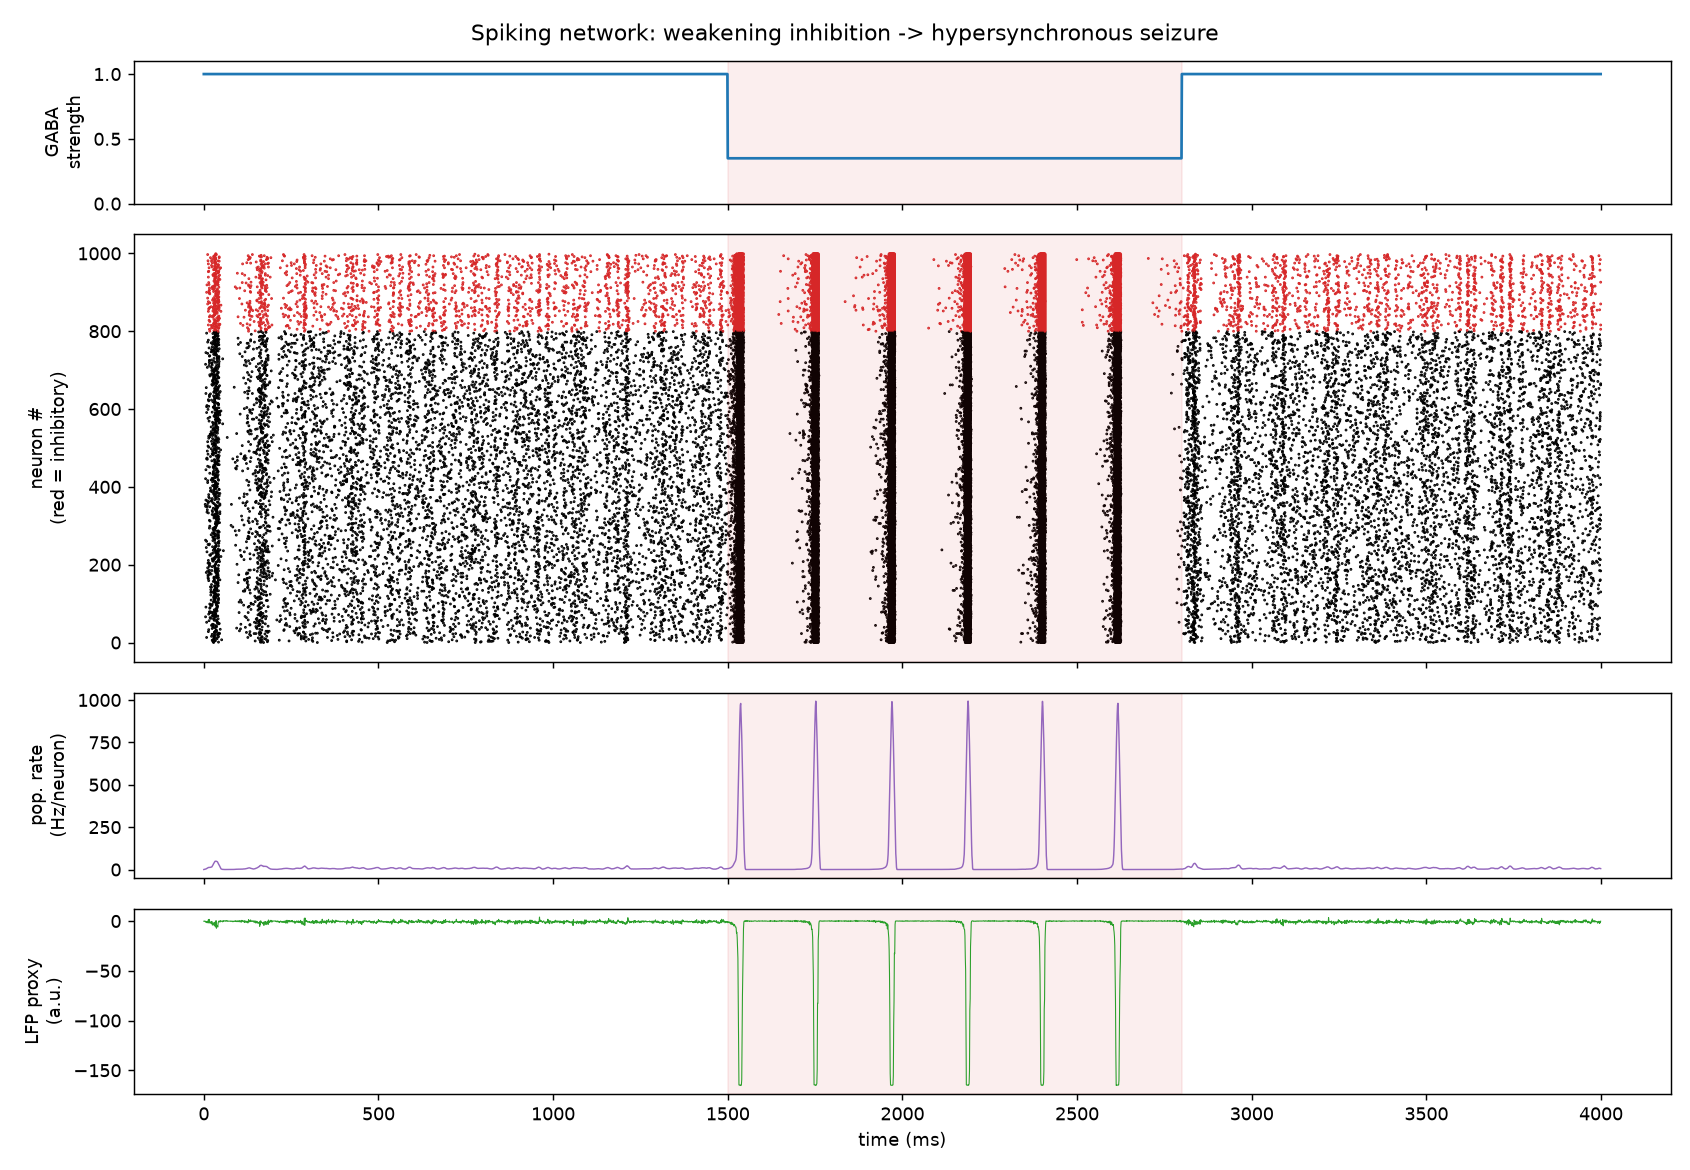
\includegraphics[width=0.78\linewidth]{epilepsy_sim/output/network_seizure.png}
\caption{Model 1: weakening inhibition turns asynchronous firing into lock-step population bursts.}
\label{fig:net}
\end{figure}

\subsection{Model 2: the Epileptor}

The Epileptor (Jirsa et al.\ 2014), the engine of The Virtual Brain, has two fast oscillators, a slow permittivity variable $z$ and a coupling term $g$:
\begin{align}
\dot x_1 &= y_1 - f_1(x_1,x_2) - z + I_1, & \dot y_1 &= y_0 - 5x_1^2 - y_1,\\
\dot z &= \tfrac{1}{\tau_0}\big(4(x_1-x_0) - z\big), & \dot x_2 &= -y_2 + x_2 - x_2^3 + I_2 + 2g - 0.3(z-3.5),\\
\dot y_2 &= \tfrac{1}{\tau_2}\big(-y_2 + f_2(x_2)\big), & \dot g &= -0.01\,(g - 0.1x_1).
\end{align}
With $x_0=-1.6$ the model produced 3 seizures in 6,000 time units (51.6\% of time ictal); with $x_0=-2.2$ (``healthy'') it produced none.

\begin{figure}[H]
\centering
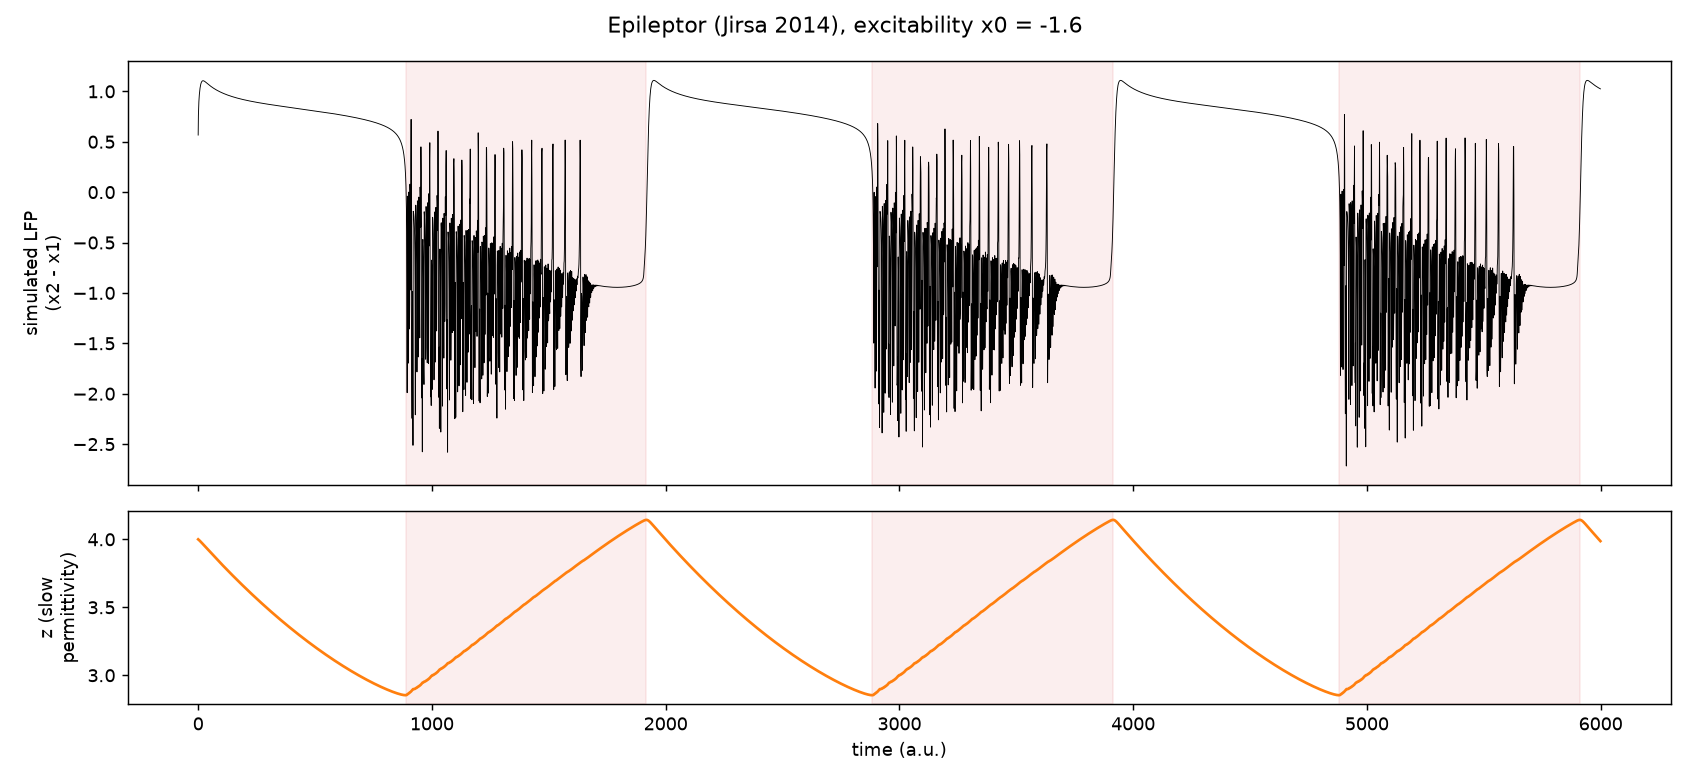
\includegraphics[width=0.78\linewidth]{epilepsy_sim/output/epileptor_seizures.png}
\caption{Model 2: Epileptor seizures driven by the slow variable $z$.}
\end{figure}

\subsection{Model 3: the ionic seizure model}

\subsubsection{Architecture and feedback loops}

A seizure is modelled as a contest between fast positive and slow negative feedback: \Kp{} accumulation depolarises neurons (+, 0.1--5\,s); \Clm{} loading makes GABA depolarising (+, 1--30\,s); KCC2 extrudes \Kp{} together with \Clm{} (+, seconds); \Nap{} accumulation drives an electrogenic pump current and a \Nap-activated \Kp{} current (Slack) ($-$); pump ATP use produces adenosine that opens GIRK channels and reduces release ($-$, 5--60\,s); glia, diffusion and vasculature clear \Kp{} ($-$).

The network has 100 neurons on a ring (every fifth inhibitory: 80 E, 20 I), local random wiring within $\pm$10 cells ($p=0.6$ from E, $0.8$ from I), a private extracellular micro-compartment per cell coupled by lateral \Kp{} diffusion, and Poisson background excitation. State variables per neuron are $V$, gates $n,h$, $[\mathrm{Ca}]_i$, \Ko, \Nai, \Cli, $g_e$, $g_i$, vesicle resources $x$ (optional depression) and adenosine $A$; $[\mathrm{K}]_i = 158-[\mathrm{Na}]_i$ and $[\mathrm{Na}]_o = 144-\beta([\mathrm{Na}]_i-18)$.

\subsubsection{Equations}

Membrane (positive-outward convention):
\begin{equation}
C\frac{dV}{dt} = -\big(I_{Na} + I_K + I_{Cl} + I_{AMPA} + I_{GABA} + s_p I_{pump}\big),
\end{equation}
with intrinsic currents (Cressman 2009)
\begin{align}
I_{Na} &= g_{Na} m_\infty^3 h (V-E_{Na}) + g_{NaL}(V-E_{Na}),\\
I_K &= \Big(g_K n^4 + g_{AHP}\tfrac{[\mathrm{Ca}]_i}{1+[\mathrm{Ca}]_i} + g_{KNa}w_\infty([\mathrm{Na}]_i) + g_{GIRK}(A)\Big)(V-E_K) + g_{KL}(V-E_K),\\
I_{Cl} &= g_{ClL}(V-E_{Cl}),
\end{align}
classical Hodgkin--Huxley rates with $m$ at steady state and $\phi=3$. Reversal potentials use $RT/F=26.64$\,mV (Cressman's value, 36\,\textdegree C):
\begin{equation}
E_K = 26.64\ln\frac{[\mathrm{K}]_o}{[\mathrm{K}]_i},\quad
E_{Cl} = 26.64\ln\frac{[\mathrm{Cl}]_i}{[\mathrm{Cl}]_o},\quad
E_{GABA} = 0.8E_{Cl} + 0.2E_{HCO_3},\quad E_{HCO_3}\approx-12.9\ \mathrm{mV}.
\end{equation}
Synapses are exponential conductances ($\tau_{AMPA}=5$\,ms, $\tau_{GABA}=8$\,ms) split by ion so that they feed the concentration equations:
\begin{equation}
I_{AMPA} = 0.64g_e(V-E_{Na}) + 0.36g_e(V-E_K),\qquad I_{GABA} = 0.8g_i(V-E_{Cl}) + 0.2g_i(V-E_{HCO_3}).
\end{equation}
Pump, glia, diffusion and KCC2 (fluxes in mM/s; corrected ModelDB version):
\begin{align}
I_{pump} &= \frac{\rho}{1+e^{(25-[\mathrm{Na}]_i)/3}}\cdot\frac{1}{1+e^{5.5-[\mathrm{K}]_o}},\quad
I_{glia} = \frac{s_g G_{glia}}{1+e^{(18-[\mathrm{K}]_o)/2.5}},\quad
I_{diff} = s_c\varepsilon([\mathrm{K}]_o - K_{bath}),\\
J_{KCC2} &= s_k U_{KCC2}\ln\frac{[\mathrm{K}]_i[\mathrm{Cl}]_i}{[\mathrm{K}]_o[\mathrm{Cl}]_o}.
\end{align}
Concentrations ($\gamma=0.0445$ current-to-concentration, $\beta=7$ volume ratio, $\div1000$ for ms$\to$s):
\begin{align}
\frac{d[\mathrm{K}]_o}{dt} &= \tfrac{1}{1000}\big(\gamma\beta(I_K+I_{AMPA,K}) - 2\beta I_{pump} - I_{glia} - I_{diff} + \beta J_{KCC2}\big) + D_{lat}\nabla^2[\mathrm{K}]_o,\\
\frac{d[\mathrm{Na}]_i}{dt} &= \tfrac{1}{1000}\big(-\gamma(I_{Na}+I_{AMPA,Na}) - 3I_{pump}\big),\qquad
\frac{d[\mathrm{Cl}]_i}{dt} = \tfrac{1}{1000}\big(\gamma(I_{Cl}+I_{GABA,Cl}) - J_{KCC2}\big).
\end{align}
The electrogenic pump current is $I^{(\mu A/cm^2)}_{pump} = s_p I_{pump}/\gamma$. The Slack current uses the Compte et al.\ (2003) curve with its EC50 shifted from 38.7 to 68.6\,mM to match this model's resting \Nai: $w_\infty = 0.37/(1+(68.6/[\mathrm{Na}]_i)^{3.5})$. Adenosine is produced in proportion to pump ATP use above rest and cleared with $\tau_A=20$\,s:
\begin{equation}
\frac{dA}{dt} = \alpha_A\max(I_{pump}-0.25,0) - \frac{A}{\tau_A},\qquad g_{GIRK} = g_{ado}\frac{A}{1+A},\qquad \text{release}\times\frac{1}{1+A}.
\end{equation}
Neurovascular coupling uses the Balloon--Windkessel model (Friston et al.\ 2000) driven by $u = k\ln(\mathrm{rate}/\mathrm{baseline})$ clipped to $[0.3\times,30\times]$:
\begin{equation}
\dot s = u - \kappa s - \gamma_f(f-1),\quad \dot f = s,\quad \tau_0\dot v = f - v^{1/\alpha},\quad
\tau_0\dot q = \frac{f(1-(1-E_0)^{1/f})}{E_0} - v^{1/\alpha}\frac{q}{v},
\end{equation}
with CBF $=f$, HbT $\propto v$, HbR $\propto q$ and HbO $=(\mathrm{HbT}-0.4\,\mathrm{HbR})/0.6$.

\subsubsection{Parameters}

\begin{table}[H]
\centering\small
\caption{Main parameters of the ionic model and their sources.}
\begin{tabularx}{\linewidth}{@{}l l L@{}}
\toprule
Parameter & Value & Source / rationale \\
\midrule
$g_{Na}, g_K, g_{AHP}$ & 100, 40, 0.01 mS/cm\textsuperscript{2} & Cressman 2009 Table 1 \\
$g_{NaL}, g_{KL}, g_{ClL}$ & 0.0175, 0.05, 0.05 mS/cm\textsuperscript{2} & Cressman 2009 \\
$\gamma$, $\beta$ & 0.0445, 7 & ModelDB code (corrected by the 2011 erratum) \\
$\rho$, $G_{glia}$ & 1.25, 66.7 mM/s & Cressman 2009 \\
$\varepsilon$, $K_{bath}$ & 1.33 s\textsuperscript{$-1$}, 4 mM & Cressman code; plasma \Kp \\
$D_{lat}$ & 0.625 s\textsuperscript{$-1$} & $D=2.5\times10^{-6}$ cm\textsuperscript{2}/s, $\Delta x=20$ \textmu m \\
$[\mathrm{Cl}]_o$, $[\mathrm{HCO_3}]_{i/o}$ & 130, 16/26 mM & Standard physiology \\
$U_{KCC2}$ & 0.4 mM/s & Gives resting \Cli{} $\approx$5--6 mM, \EGABA{} $\approx-70$ mV \\
$g_{KNa}$ & 1.33 mS/cm\textsuperscript{2}, EC50 68.6 mM & Compte 2003, shifted \\
$g_{ado}, \alpha_A, \tau_A$ & 0.3 mS/cm\textsuperscript{2}, 0.5, 20 s & During \& Spencer 1992; Boison \\
Recurrent $g_E/g_I$ & 1.3 / 2.6 mS/cm\textsuperscript{2} & Balanced E/I, calibrated \\
Background & 60 Hz $\times$ 0.07 mS/cm\textsuperscript{2} & 4--6 Hz asynchronous baseline \\
Pump-current scale $s_p$ & 1.0 & See calibration log \\
Neurovascular gain $k$ & 0.12 & CBF rise of $\approx$+40--100\% \\
\bottomrule
\end{tabularx}
\end{table}

\subsubsection{Healthy vs epileptic tissue and numerics}

Both tissues share neurons and wiring; only the pathology, modelled on hippocampal sclerosis, differs: KCC2 $\times$0.3 (downregulated in human epileptic tissue), glial \Kp{} buffering $\times$0.3 (Kir4.1 loss) and vascular \Kp{} clearance $\times$0.35 (gliosis). Each run first settles for a 60\,s warm-up; at $t=10$--12\,s both receive the same 2\,s trigger (+400\,Hz excitatory input). Voltage and gates use exponential Euler, $V_{t+dt} = V_\infty + (V_t - V_\infty)e^{-dt\,g_{tot}}$, which stays stable when conductances become large (forward Euler produced NaN); $dt=0.02$\,ms; concentrations use forward Euler; the loop is numba-compiled (100 neurons $\times$ 360\,s in $\approx$6\,min).

\subsubsection{Validation}

With all additions switched off (fixed \Clm, no pump current, no $I_{KNa}$, no adenosine), a single neuron in 8\,mM bath \Kp{} reproduces Cressman et al.\ (2009) Fig.~1:

\begin{table}[H]
\centering\small
\caption{Validation against Cressman et al.\ 2009, Fig.~1.}
\begin{tabular}{@{}lll@{}}
\toprule
Quantity & Cressman 2009 & This implementation \\
\midrule
Seizure-like events & Periodic, every $\approx$30 s & Every $\approx$29.5 s \\
\Ko{} range & $\approx$6.7$\to$10.2 mM & 6.7$\to$10.7 mM \\
\Nai{} range & $\approx$16.3$\to$19 mM & 15.5$\to$19.1 mM \\
\bottomrule
\end{tabular}
\end{table}

\begin{figure}[H]
\centering
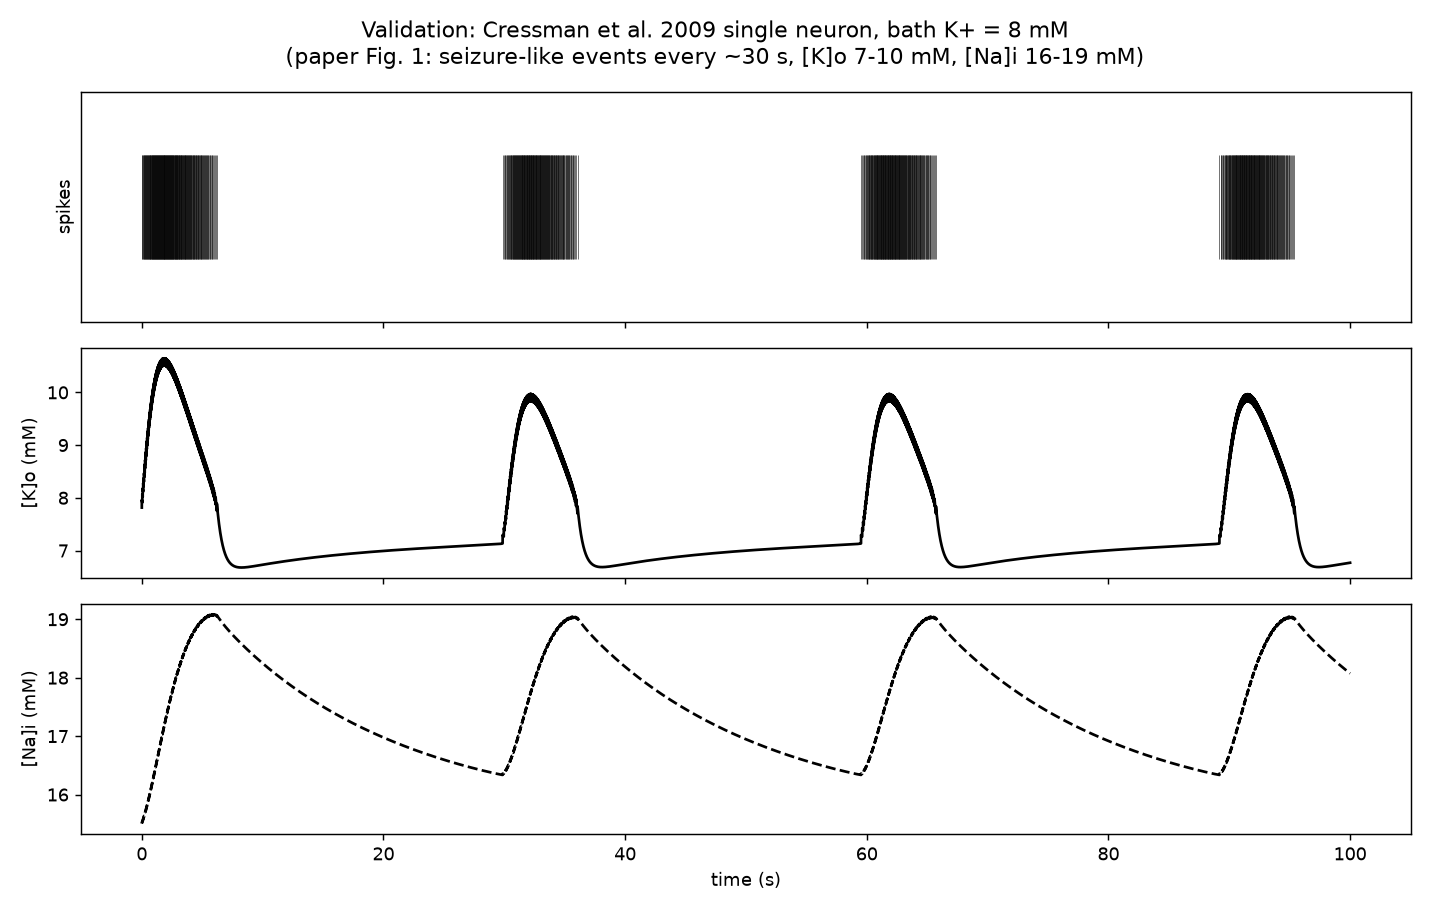
\includegraphics[width=0.7\linewidth]{epilepsy_sim/output/ionic_validation.png}
\caption{Single-neuron validation against Cressman et al.\ 2009, Fig.~1.}
\end{figure}

\subsubsection{Results}

\begin{table}[H]
\centering\small
\caption{Healthy vs epileptic tissue (same neurons, wiring and trigger).}
\label{tab:ionic}
\begin{tabularx}{\linewidth}{@{}l l l L@{}}
\toprule
Measure & Healthy & Epileptic & Real-world reference \\
\midrule
Baseline E firing & 6.1 Hz & 17.3 Hz & Hyperexcitable cortex \\
Resting \Cli{} & 5.6 mM & \best{11.6 mM} & Elevated in human epileptic tissue \\
Resting \EGABA{} (chord) & $-69.6$ mV & \best{$-54.1$ mV} & Depolarised with KCC2 loss \\
Resting \Ko{} & 4.18 mM & 4.59 mM & Impaired buffering \\
Interictal discharges & not epileptiform & \best{33/min} & IEDs on EEG \\
Peak \Ko{} (trigger) & 6.1 mM & \best{12.2 mM} & Ictal \Kp{} ceiling $\approx$10--12 mM \\
Peak \Cli{} & 7.4 mM & \best{15.2 mM} & Ictal \Clm{} loading \\
Peak \EGABA{} & $-63.7$ mV & \best{$-48.3$ mV} & Depolarising GABA \\
Peak \Nai{} & 26.2 mM & 29.8 mM & Ictal \Nap{} loading \\
Peak adenosine & 0.12 & \best{0.68} & Ictal adenosine surge \\
Postictal silence & 13.7 s & \best{25 s} & Postictal depression \\
Minimum \Ko{} after & 3.88 mM & \best{3.66 mM} & Postictal \Kp{} undershoot \\
CBF peak $\to$ minimum & +42\% $\to$ $-47$\% & +31\% $\to$ $-46$\% & Hyperperfusion then hypoperfusion \\
\bottomrule
\end{tabularx}
\end{table}

In epileptic tissue the interictal state shows synchronous population bursts at $\approx$33/min, each sending local \Ko{} to 7--9\,mM with a saw-tooth in \Cli. The trigger drives \Ko{} to the 12\,mM ceiling, \Cli{} to 15.2\,mM (\EGABA{} $-48.3$\,mV, inhibition collapsed), the pump to $\approx$1\,mM/s and adenosine to 0.68 (5.7$\times$ healthy). A 25\,s postictal silence follows with a \Kp{} undershoot to 3.66\,mM (as predicted by Krishnan \& Bazhenov 2011) and CBF falls to $-46$\% (postictal hypoperfusion). The healthy tissue caps \Ko{} near 6\,mM and recovers after a 13.7\,s pump after-hyperpolarisation. The CBF peak is smaller in epileptic tissue because its baseline is already hyperactive.

\begin{figure}[H]
\centering
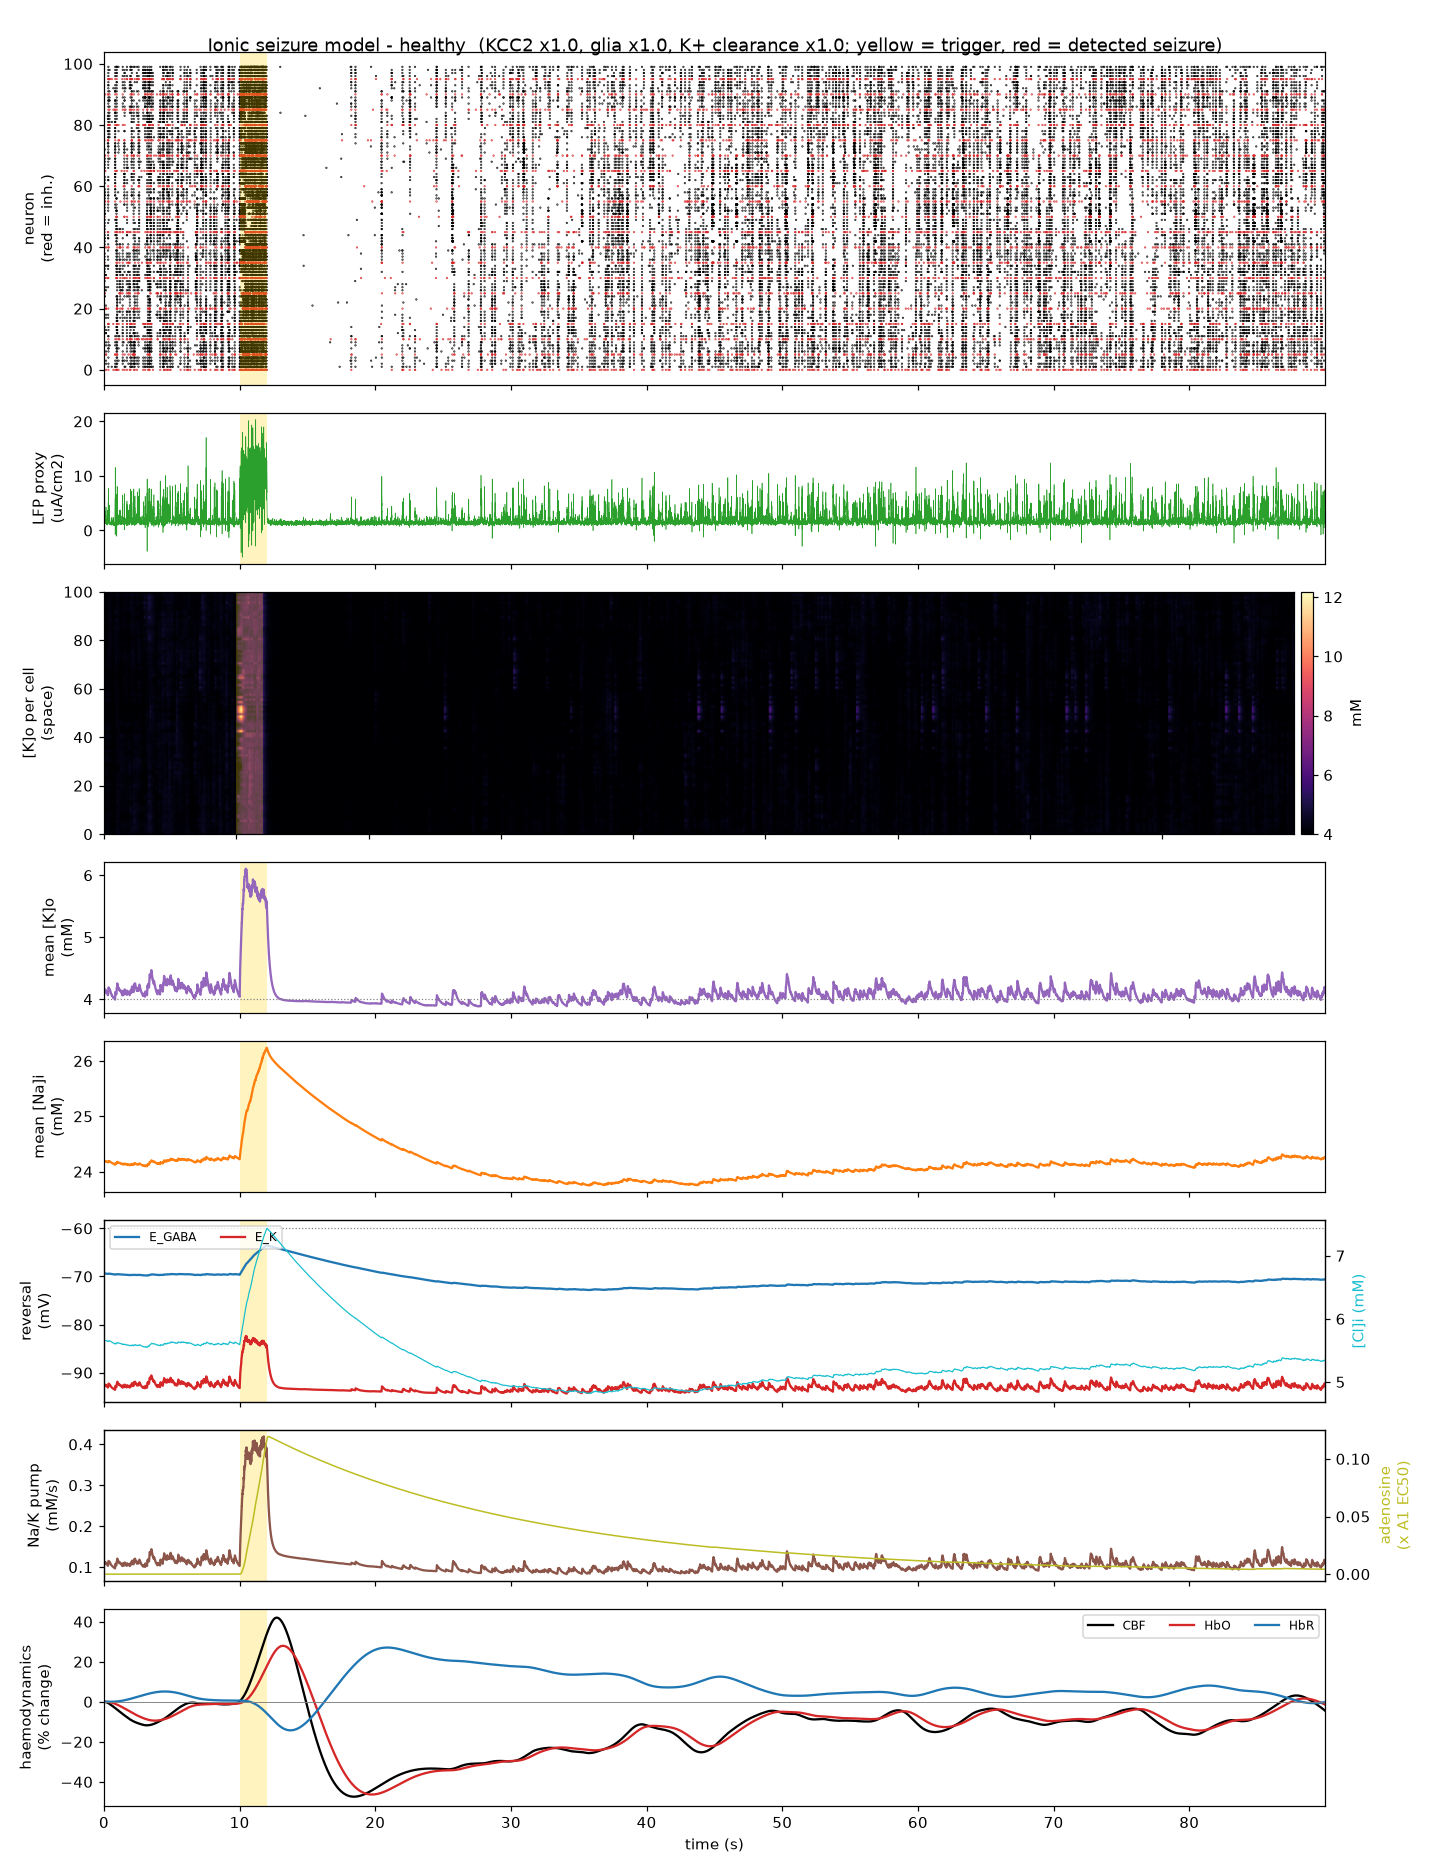
\includegraphics[width=0.49\linewidth]{epilepsy_sim/output/ionic_healthy.png}
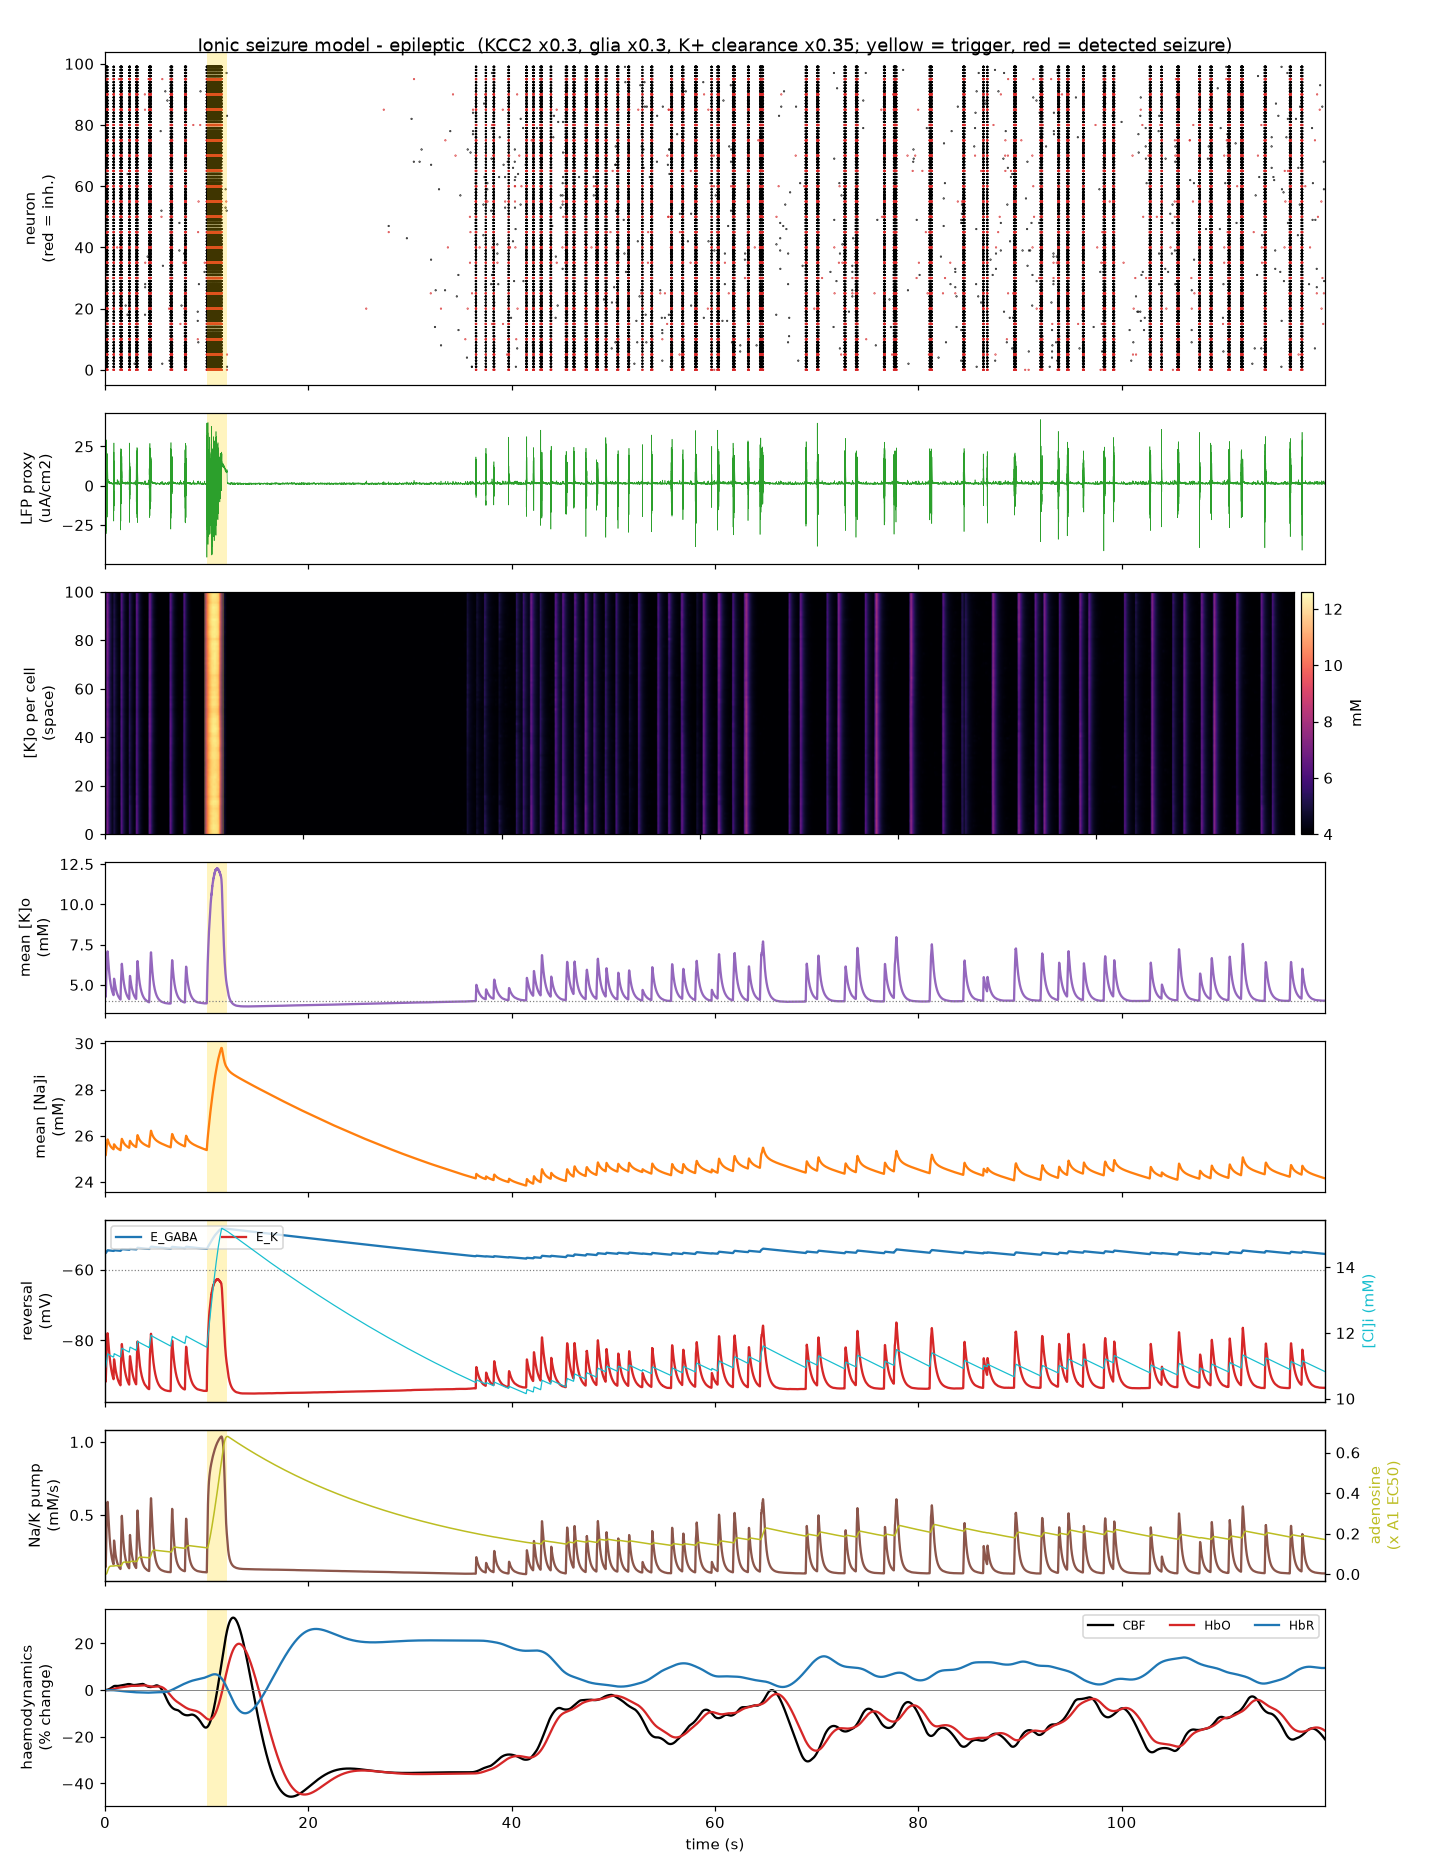
\includegraphics[width=0.49\linewidth]{epilepsy_sim/output/ionic_epileptic.png}
\caption{Ionic model, healthy (left) and epileptic (right): raster, LFP proxy, space--time \Ko{} map, mean \Ko, \Nai, \EGABA/$E_K$/\Cli, pump flux and adenosine, CBF/HbO/HbR.}
\end{figure}

\paragraph{Corrections recorded.} (1) The first E\textsubscript{GABA} values printed ($-70.7$, $-66$, $-57.7$, $-52$\,mV) came from a diagnostic using the GHK form, not the chord form the simulated current obeys; recomputed chord values are $-69.6$, $-63.7$, $-54.1$ and $-48.3$\,mV. The dynamics were unaffected and the code now records the chord form. (2) The healthy ``silence'' metric first printed 0.0\,s because the smoothing window still contained the trigger; the corrected metric searches from 1\,s after the trigger and gives 13.7\,s. (3) The healthy ``36 discharges'' are threshold crossings by normal fluctuations; only rates should be compared.

\subsubsection{Calibration log}

\begin{longtable}{@{}p{0.4cm} p{3.9cm} p{4.6cm} p{5.6cm}@{}}
\caption{Development log: how the ionic model was calibrated.}\\
\toprule
\# & Symptom & Diagnosis & Fix \\
\midrule
\endfirsthead
\toprule
\# & Symptom & Diagnosis & Fix \\
\midrule
\endhead
1 & Printed Cressman equations gave wrong dynamics & Typographical errors in the paper's concentration equations & Used the ModelDB C code ($\gamma=0.0445$, $\div1000$, $\beta$ on $I_K$) per the 2011 erratum \\
2 & -- & Validation & Reproduced Cressman Fig.~1 \\
3 & Baseline firing 245 Hz & One background AMPA event moved $V$ by $\approx$50 mV (tiny leak conductance) & Recalibrated background to 60 Hz $\times$ 0.02 mS/cm\textsuperscript{2} ($\approx$3 Hz) \\
4 & Network locked into permanent 100--200 Hz firing & \Nai{} pinned at 32 mM, no termination & Added electrogenic pump current and \Nap-activated \Kp{} current (Krishnan \& Bazhenov; Compte) \\
5 & E cells silent while I cells fire & Compte's curve assumes resting \Nai{} $\approx$11 mM; here $\approx$19.5 mM & Shifted EC50 38.7$\to$68.6 mM \\
6 & \Nai{} drifting upward & Start state not steady & 60 s warm-up \\
7 & Epileptic tissue did not seize & \Kp{} clearance too fast & Pathology includes glia $\times$0.3 and clearance $\times$0.35 as well as KCC2 loss \\
8 & NaN crash at seizure-level activity & Forward Euler unstable & Exponential Euler (a sign bug in its first version, $v_\infty = v_i + dv/g_{tot}$, was fixed and re-validated) \\
9 & Seizures never terminated & Sustained by depolarising GABA & Tried Tsodyks--Markram depression (U = 0.07, $\tau$ = 700 ms) \\
10 & With depression: no seizures or a 30--50 Hz steady state & Depression caps drive, no slow brake & Depression made optional; adenosine added \\
11 & Per-spike adenosine damped even baseline & Unphysiological & Adenosine proportional to pump ATP use above rest \\
12 & Healthy vs epileptic clearly different & -- & Adopted as default \\
13 & Ictal event stops with the trigger & Pump after-hyperpolarisation 30 mV vs 1--10 mV measured & \code{--pump-i}: at 0.15 seizures self-sustain (10--20 s), self-terminate and recur, but healthy tissue becomes bistable (Gulledge 2013) \\
14 & Sweep at \code{--pump-i 0.35} & Stopped (machine ran low on memory) & Open \\
\bottomrule
\end{longtable}

\subsubsection{Mapping onto real seizure biology, optical readout and limitations}

The model reproduces the ictal \Kp{} ceiling, chloride loading, KCC2 loss, KCC2-mediated \Kp{} loading, interictal discharges, \Nap{} accumulation and pump activation, the adenosine surge, postictal depression, the postictal \Kp{} undershoot, ictal hyperperfusion followed by hypoperfusion, and spatial spread by lateral diffusion; it does \emph{not} yet produce a self-sustained 30--120\,s focal seizure at the default pump setting, and loss of consciousness or motor signs are out of scope. Its bottom panel is what an optical sensor would record: a CBF/HbO surge delayed by seconds during the event and a dip below baseline afterwards; brief interictal events are nearly invisible optically, so optics alone would miss them, while EEG plus optics gives the full picture. Limitations: ictal events are not self-sustaining at default settings; a tiny 1-D network without dendrites, layers, thalamus or long-range connections; one neuron type per population; simplified conservation (no cell swelling); energy implicit (no ATP/O\textsubscript{2}); generic haemodynamics without an initial dip; an LFP proxy rather than a volume-conductor EEG; a simple threshold IED counter; not a clinical tool.

% ============================================================================
\section{Inferring hidden brain variables from non-invasive signals}
\label{sec:inference}

\subsection{Measured vs inferred}

Several variables in Table~\ref{tab:ionic} (intracellular chloride, extracellular potassium, adenosine, KCC2 strength) can only be \emph{measured} with probes inside brain tissue (ion-selective microelectrodes, perforated-patch clamp, genetically encoded sensors, microdialysis). A wearable can only \emph{infer} them: compute the most likely value, with an uncertainty, from signals it can record plus a model that explains how the hidden quantity produces those signals. The question ``can invasive measurements be converted to non-invasive ones?'' was answered in these terms, and ``inferred'' was defined as \emph{calculated, not measured; as good as the model; always reported with uncertainty}.

\begin{table}[H]
\centering\small
\caption{Which seizure variables need inference (values from the ionic model).}
\begin{tabularx}{\linewidth}{@{}l l l L l@{}}
\toprule
Variable & Healthy & Epileptic & Gold standard (invasive) & Non-invasive? \\
\midrule
Resting \Cli & 5.6 mM & 11.6 mM & 2-photon imaging of Cl\textsuperscript{--} sensors & Infer \\
Resting \EGABA & $-69.6$ mV & $-54.1$ mV & Gramicidin perforated patch & Infer (TMS-EEG proxy) \\
Interictal discharges & -- & 33/min & Intracranial EEG & Scalp/ear EEG \\
Peak \Ko & 6.1 mM & 12.2 mM & \Kp-selective microelectrodes & DC-EEG proxy, infer \\
Adenosine surge & 0.12 & 0.68 & Microdialysis, biosensors & Infer \\
Blood flow & +42\% $\to$ $-47$\% & +31\% $\to$ $-46$\% & Laser Doppler, SPECT, fMRI & fNIRS, DCS, PPG \\
\bottomrule
\end{tabularx}
\end{table}

\subsection{General framework}

A forward model maps hidden quantities $\boldsymbol\theta$ (KCC2 strength, \Cli, \Ko, adenosine) to sensor measurements $\mathbf y$ (EEG discharge rate, DC shift, 1/$f$ slope, HbO/HbR) with noise: $\mathbf y = f(\boldsymbol\theta)+\boldsymbol\varepsilon$. Inversion uses Bayes' theorem,
\begin{equation}
P(\boldsymbol\theta\mid\mathbf y) = \frac{P(\mathbf y\mid\boldsymbol\theta)P(\boldsymbol\theta)}{P(\mathbf y)}.
\end{equation}
With Gaussian noise $\varepsilon_i\sim\mathcal N(0,\sigma_i^2)$,
\begin{equation}
\ln P(\mathbf y\mid\boldsymbol\theta) = \mathrm{const} - \frac12\sum_i\frac{(y_i-f_i(\boldsymbol\theta))^2}{\sigma_i^2},
\end{equation}
so with a flat prior the maximum a posteriori estimate is weighted least squares, $\hat{\boldsymbol\theta} = \arg\min\sum_i((y_i-f_i(\boldsymbol\theta))/\sigma_i)^2$; an informative prior adds $-2\ln P(\boldsymbol\theta)$. Uncertainty is the posterior mean and variance, reported as $\bar\theta\pm2\sigma_\theta$. Time-varying hidden states are tracked with a Kalman filter,
\begin{align}
\hat x_t^- &= F\hat x_{t-1},\quad P_t^- = FP_{t-1}F^\top + Q,\quad K_t = P_t^-H^\top(HP_t^-H^\top+R)^{-1},\\
\hat x_t &= \hat x_t^- + K_t(y_t - H\hat x_t^-),\quad P_t = (I-K_tH)P_t^-,
\end{align}
or its unscented/extended variants for nonlinear models (Ullah \& Schiff 2010 reconstructed hidden \Ko{} during seizures with a UKF). When the likelihood cannot be written down, approximate Bayesian computation draws $\theta^*$ from the prior, simulates $y^*=f(\theta^*)$ and accepts candidates whose output is close to the data; the Virtual Epileptic Patient uses such simulation-based methods to infer epileptogenicity from SEEG and MRI.

\subsection{Formulas for each quantity}

\paragraph{Nernst.} Equal electrochemical potential across the membrane gives $E_X = \frac{RT}{zF}\ln\frac{[X]_{out}}{[X]_{in}}$. $RT/F$ is 26.64\,mV at 36\,\textdegree C (the value in Cressman's model; 61.34\,mV/decade) and 26.73\,mV at 37\,\textdegree C (61.54\,mV/decade).

\paragraph{Extracellular \Kp{} from a glial electrode.} Glial membranes behave like \Kp{} electrodes but not perfectly Nernstian: $\Delta V_{glia} = S\log_{10}([\mathrm K]_{o,new}/[\mathrm K]_{o,rest})$, hence
\begin{equation}
[\mathrm K]_{o,new} = [\mathrm K]_{o,rest}\cdot10^{\Delta V_{glia}/S},
\end{equation}
with measured slopes of 61.5 (theory), $\approx$Nernstian (amphibian), \textbf{51} (mammalian primary glia) and 40\,mV/decade (C6 line).

\paragraph{\Kp{} from a scalp DC shift: no closed form.} The scalp DC shift is a field potential produced by currents through the glial syncytium, of opposite polarity to glial membrane voltage, attenuated to roughly 7\% by skull, CSF and dura and dependent on geometry and conductivity. No single constant converts scalp \uV{} to mM; the correct approach is model-based tracking with \Ko{} as a hidden state. It remains a strong qualitative marker of seizure onset.

\paragraph{Intracellular chloride from \EGABA.} The chord-conductance form (used by \code{ionic.py}) follows from zero net current through parallel Cl\textsuperscript{--} and \HCO{} conductances:
\begin{align}
E_{GABA} &= \frac{g_{Cl}E_{Cl}+g_{HCO_3}E_{HCO_3}}{g_{Cl}+g_{HCO_3}} = 0.8E_{Cl}+0.2E_{HCO_3},\\
\Rightarrow\quad E_{Cl} &= \frac{E_{GABA}-0.2E_{HCO_3}}{0.8},\qquad [\mathrm{Cl}]_i = [\mathrm{Cl}]_o\exp\!\left(\frac{E_{Cl}}{RT/F}\right).
\end{align}
Worked check at epileptic rest: $E_{GABA}=-54.1$\,mV and $E_{HCO_3}=26.64\ln(16/26)=-12.9$\,mV give $E_{Cl}=-64.4$\,mV and $[\mathrm{Cl}]_i = 130e^{-64.4/26.64}=11.6$\,mM. The GHK (permeability) form,
\begin{align}
E_{GABA} &= \frac{RT}{F}\ln\frac{P_{Cl}[\mathrm{Cl}]_i+P_{HCO_3}[\mathrm{HCO_3}]_i}{P_{Cl}[\mathrm{Cl}]_o+P_{HCO_3}[\mathrm{HCO_3}]_o},\\
\Rightarrow\quad [\mathrm{Cl}]_i &= ([\mathrm{Cl}]_o + r[\mathrm{HCO_3}]_o)\,e^{E_{GABA}/(RT/F)} - r[\mathrm{HCO_3}]_i,
\end{align}
with $r=P_{HCO_3}/P_{Cl}$ measured at 0.2--0.44, gives different values for the same chloride:

\begin{table}[H]
\centering\small
\caption{Chord vs GHK \EGABA{} for the same chloride levels.}
\begin{tabular}{@{}lcccc@{}}
\toprule
State & \Cli{} (mM) & $E_{Cl}$ (mV) & Chord \EGABA & GHK \EGABA{} ($r=0.25$) \\
\midrule
Healthy rest & 5.6 & $-83.8$ & $-69.6$ & $-70.7$ \\
Healthy peak & 7.4 & $-76.4$ & $-63.7$ & $-66.1$ \\
Epileptic rest & 11.6 & $-64.4$ & $-54.1$ & $-57.8$ \\
Epileptic peak & 15.2 & $-57.2$ & $-48.3$ & $-52.3$ \\
\bottomrule
\end{tabular}
\end{table}

\EGABA{} itself would come non-invasively from TMS-EEG paired-pulse inhibition (SICI/LICI) plus model inversion, which carries its own uncertainty.

\paragraph{Excitation/inhibition balance from the EEG spectrum.} The aperiodic component is fitted with specparam/FOOOF, $L(f) = b - \log_{10}(k+f^\chi)$ (knee) or $b-\chi\log_{10}f$ (fixed). Summed exponentially decaying synaptic currents have a Lorentzian spectrum; Gao et al.\ (2017) showed that the 30--50\,Hz exponent $\chi$ tracks E/I (higher $\chi$ = more inhibition). It gives relative, not absolute, balance.

\paragraph{Adenosine: no simple formula.} An earlier draft proposed $A_{peak} = A_{th}e^{T_{silence}/\tau_A}$. The simulation's own data require thresholds of 0.195 (epileptic: $A_{peak}=0.68$, $T=25$\,s) and 0.093 (healthy), differing 2$\times$; postictal silence is not set by adenosine alone (the pump current contributes), so the formula was withdrawn. Adenosine can only be inferred by fitting the full model.

\paragraph{Haemoglobin from optics (modified Beer--Lambert law).} $OD = -\log_{10}(I/I_0) = \varepsilon cL + G$; in tissue $L = d\cdot DPF$ and $G$ cancels in a change:
\begin{equation}
\Delta OD(\lambda) = \big(\varepsilon_{HbO}(\lambda)\Delta[\mathrm{HbO}] + \varepsilon_{HbR}(\lambda)\Delta[\mathrm{HbR}]\big)\,d\,DPF(\lambda),
\end{equation}
solved at two wavelengths by inverting a $2\times2$ extinction matrix. The differential pathlength factor for the adult frontal head (Scholkmann \& Wolf 2013) is
\begin{equation}
DPF(\lambda,A) = 223.3 + 0.05624A^{0.8493} - 5.723\times10^{-7}\lambda^3 + 0.001245\lambda^2 - 0.9025\lambda,
\end{equation}
giving DPF $\approx$6.3 at 760\,nm and age 30. Partial volume (the brain is only part of the light path) causes underestimation; short-channel regression or time-domain NIRS reduce scalp contamination; a temple PPG device samples mostly scalp and superficial arterial flow.

\paragraph{Joint fit.} The strongest approach fits all signals at once: $\hat{\boldsymbol\theta} = \arg\min[\sum_{signals}\sum_t((y_t-f_t(\boldsymbol\theta))/\sigma)^2 - 2\ln P(\boldsymbol\theta)]$ with $f$ = \code{ionic.py}, yielding full time courses of \Ko, \Cli, \EGABA{} and adenosine with uncertainty.

\subsection{Non-invasive routes found in the literature}

Direct nuclear MRI can map ions in a scanner (\textsuperscript{23}Na MRI and triple-quantum-filtered MRI, with raised sodium in the epileptogenic zone and 7T sodium features already used as priors; \textsuperscript{39}K MRI feasible at 7T with $\approx$1\,cm\textsuperscript{3} voxels in $\approx$30\,min; \textsuperscript{35}Cl MRI feasible but $\approx$15$\times$ weaker than sodium; 7T MRS and GluCEST for glutamate/GABA). Proxies include DC/infraslow EEG for \Kp, TMS-EEG SICI/LICI for GABA-A efficacy, the aperiodic exponent for E/I, [\textsuperscript{18}F]CPFPX PET for A1 receptors (not endogenous adenosine), and postictal suppression plus hypoperfusion for adenosine via a model. Digital twins (Virtual Epileptic Patient; neural-mass models of TMS-EEG) invert models against data. Emerging routes (photoacoustic \Kp{} imaging with injected nanoparticles; implantable ion-selective arrays) are not yet usable in humans. A practical wearable pipeline would combine DC-capable EEG, fNIRS/DCS and PPG features, optionally a one-off 7T sodium MRI as a prior, and a patient-fitted model with UKF or simulation-based inference; validation against invasive ground truth (e.g.\ patients undergoing intracranial monitoring) is mandatory.

\subsection{Verification audit}

The user asked whether we were ``100\% sure'' of the formulas; each was re-derived and checked against the literature, with numerical checks.

\begin{table}[H]
\centering\small
\caption{Verification audit of the inference formulas.}
\begin{tabularx}{\linewidth}{@{}c l l L@{}}
\toprule
\# & Formula & Verdict & Correction \\
\midrule
1 & Bayes, posterior, credible interval & Correct & -- \\
2 & Least squares = best estimate & Conditional & Only with Gaussian noise and a flat prior (derived) \\
3 & Kalman filter & Correct & UKF for nonlinear models \\
4 & Nernst 61.5 mV/decade & Correct at 37\,\textdegree C & \code{ionic.py}'s RT/F = 26.64 mV is 36\,\textdegree C; comment fixed \\
5 & $[\mathrm K]_o = [\mathrm K]_{o,rest}10^{\Delta V/61.5k}$ from scalp DC & \textbf{Wrong (oversimplified)} & Mammalian glia slope is 51; scalp DC is a field potential; attenuation not constant; replaced by glial formula + model tracking \\
6 & GHK inverse for \Cli & \textbf{Mismatch} & Valid formula, but the model's current is chord; recorded \EGABA{} values were 1--4 mV off; code and docs corrected \\
7 & Aperiodic fit & Correct & Relative E/I only \\
8 & $A_{peak}=A_{th}e^{T/\tau}$ & \textbf{Withdrawn} & Inconsistent thresholds (0.195 vs 0.093) \\
9 & MBLL, DPF $\approx$6 & Correct & Scholkmann--Wolf gives 6.3 at 760 nm, age 30 \\
\bottomrule
\end{tabularx}
\end{table}

Limitations of inference: model dependence, non-identifiability (weak KCC2 and weak GABA receptors both reduce inhibition), mandatory uncertainty reporting, propagation of parameter uncertainty (e.g.\ $r$ = 0.2--0.44, glial slope 40--59\,mV/decade), mandatory validation, and research-only status.

% ============================================================================
\section{Testing the formulas and cross-validating with The Virtual Brain}
\label{sec:twin}

The request was to build simulations using the derived formulas and one using an existing real simulator, and to compare them (\code{infer.py}, \code{tvb_compare.py}).

\subsection{Method: twin experiments with deliberate confounds}

In a twin experiment a simulator with known hidden values synthesises the signal a sensor would record, realistic confounds are added, the inference method is applied, and the result is compared with the truth. Confounds are essential; otherwise inverting the same equation is trivially perfect.

\begin{table}[H]
\centering\small
\caption{Confounds injected in the twin experiments.}
\begin{tabularx}{\linewidth}{@{}l l l L@{}}
\toprule
Confound & Used in & Value & Realism \\
\midrule
Glial slope unknown & E1 & true 51 vs textbook 61.5 mV/decade & Measured mammalian glia \\
Skull attenuation unknown & E2 & true $\alpha=0.01$, guessed 0.005 & Cortex-to-scalp gain varies \\
Electrode drift & E2 & random walk 0.4 \uV/step & DC-EEG's main practical problem \\
\EGABA{} estimation error & E3 & $\pm$2 mV & TMS-EEG estimates are indirect \\
\HCO/\Clm{} permeability & E3 & $r$ = 0.2--0.44 & Literature range \\
Scalp haemodynamics & E5 & Mayer waves 0.1 Hz + cardiac 1.2 Hz & Dominant fNIRS contaminant \\
Partial volume & E5 & 15\% of photon path in cortex & Layered head \\
Individual DPF & E5 & true DPF 10\% above formula & Inter-subject variation \\
Onset-picking noise & T2 & $\pm$20 ms & SEEG annotation \\
\bottomrule
\end{tabularx}
\end{table}

\subsection{Results E1--E7}

\paragraph{E1: \Kp{} from a glial electrode.} Textbook slope (61.54): RMSE 0.239\,mM, peak 10.29\,mM (true 12.21, $-16$\%). Measured slope (51): RMSE \textbf{0.062}\,mM, peak 12.32\,mM (+1\%). The inverse is exact only with the measured slope.

\paragraph{E2: \Kp{} from scalp DC-EEG with a Kalman filter.} The process model $d[\mathrm K]_o/dt = a\cdot\mathrm{rate} - ([\mathrm K]_o - K_0)/\tau$ was calibrated on healthy data ($a=0.093$, $\tau=0.51$\,s) and applied to epileptic data whose clearance is 3$\times$ slower. Naive constant-gain conversion: RMSE 1.41\,mM, peak \textbf{29.2}\,mM (2.4$\times$ too high). Activity-driven process model alone: 0.51\,mM (peak 14.1). EKF (process model + DC): \textbf{0.50}\,mM (peak 14.0); the EKF's skull-gain estimate was 0.015 (true 0.010). Honest finding: with unknown gain and drift the DC channel added almost nothing beyond the EEG-driven model; it would need a calibrated gain.

\paragraph{E3: \Cli{} from an \EGABA{} estimate.} Chord inverse: RMSE \textbf{1.12}\,mM, bias $-0.13$. GHK: $r=0.20$ RMSE 3.05 (bias \textbf{+2.72}); $r=0.25$ 2.50 (+2.09); $r=0.44$ 1.47 ($-0.32$, a coincidental crossing). With the right formula $\pm$2\,mV of \EGABA{} error becomes $\approx\pm$1.1\,mM, enough to separate healthy (5.6) from epileptic (11.6) tissue; the wrong formula family adds a systematic bias up to 2.7\,mM.

\paragraph{E4: E/I from the EEG spectrum.} 30--50\,Hz fixed fit: $\chi$ = 1.65 healthy ($R^2$ 0.87) vs 1.50 epileptic (0.75), the direction associated with more excitation. The broadband 2--200\,Hz knee fit failed in epileptic tissue ($\chi\approx0$, $R^2$ 0.74) because interictal spikes inject high-frequency power. $\chi$ is usable only as a relative marker, in a narrow band and outside bursts.

\paragraph{E5: HbO/HbR from fNIRS.} Naive MBLL: RMSE 10.3\,\uM, correlation 0.873, amplitude 22\%. With short-channel regression: correlation \textbf{0.996}, amplitude 16\%. With partial-volume correction: RMSE \textbf{1.40}\,\uM, amplitude 1.10 (the residual +10\% is exactly the injected DPF error). HbR, full pipeline: 0.49\,\uM, r = 0.999. A Temple-style device without a short channel and depth information would underestimate cortical flow about 5$\times$ and be contaminated by scalp physiology.

\paragraph{E6: adenosine from postictal silence.} $A_{peak}e^{-T/20}$ reproduced the true adenosine at recovery in both tissues (0.060 vs 0.061 healthy; 0.195 vs 0.196 epileptic), so the decay law is exact, but the level at which firing resumes differs 3.2$\times$ between tissues; a universal threshold does not exist, confirming the withdrawal.

\paragraph{E7: KCC2 strength by Bayesian grid inference.} Observed features: resting \EGABA{} ($\pm$1.5\,mV) and mean excitatory rate ($\pm$25\%); six ionic runs at different KCC2 strengths.

\begin{table}[H]
\centering\small
\caption{E7: posterior over KCC2 strength (true 0.3).}
\begin{tabular}{@{}lcccccc@{}}
\toprule
KCC2 ($\times$ normal) & 0.15 & 0.2 & \textbf{0.3} & 0.45 & 0.7 & 1.0 \\
\midrule
Simulated \EGABA{} (mV) & $-51.3$ & $-52.5$ & $-54.2$ & $-56.4$ & $-60.7$ & $-63.5$ \\
Simulated E rate (Hz) & 13.2 & 12.4 & 9.9 & 12.2 & 10.3 & 10.9 \\
Posterior & 0.014 & 0.103 & \textbf{0.414} & \textbf{0.468} & 0.001 & $\approx$0 \\
\bottomrule
\end{tabular}
\end{table}

Posterior mean \textbf{0.36$\pm$0.09} (true 0.30); the MAP fell on 0.45 because the noisy \EGABA{} ``measurement'' was $-55.3$ vs $-54.0$\,mV. \EGABA{} carries almost all the information (rate is non-monotonic in KCC2); healthy and severe-loss values are correctly ruled out, 0.3 vs 0.45 honestly not.

\begin{figure}[H]
\centering
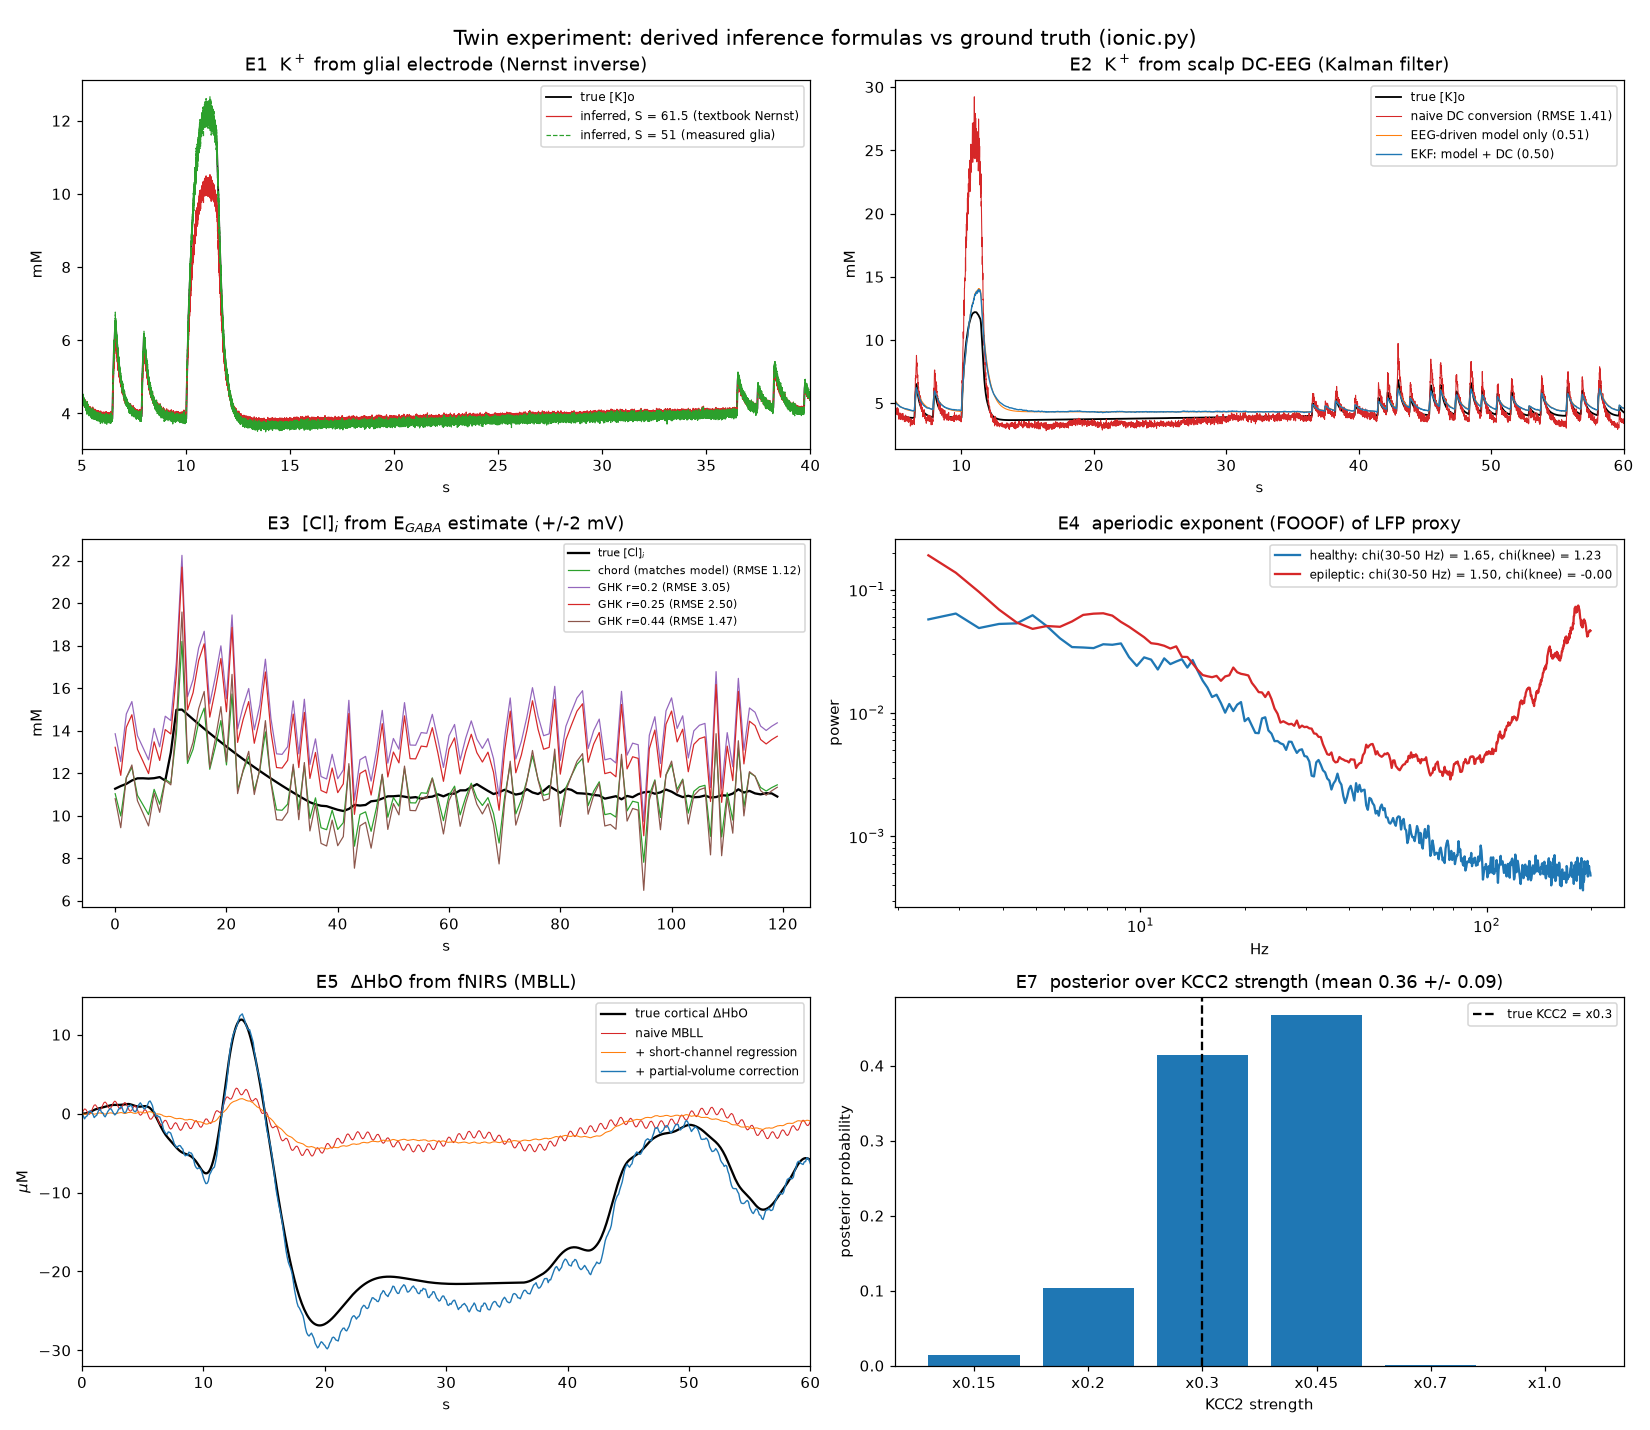
\includegraphics[width=0.85\linewidth]{epilepsy_sim/output/infer_results.png}
\caption{Twin experiments E1--E7.}
\end{figure}

\subsection{The Virtual Brain}
\label{sec:tvb}

\paragraph{T1: our Epileptor vs TVB's official Epileptor.} Same equations (checked line by line against TVB's source), parameters ($x_0=-1.6$, $I_{ext}=3.1$, $r=1/2857$) and initial state.

\begin{table}[H]
\centering\small
\caption{T1 cross-validation.}
\begin{tabular}{@{}llll@{}}
\toprule
& TVB (Heun, dt 0.05) & Ours (Euler, dt 0.05) & Ours (Euler, dt 0.01) \\
\midrule
Seizures in 6000 a.u. & 3 & 3 & 3 \\
Onsets & 886.2, 2820.2, 4754.2 & 887.0, 2883.0, 4880.0 & \textbf{886.2}, 2827.6, 4769.0 \\
Seizure duration & 968.7 & 1030 & \textbf{976.2} \\
$z$ RMSE vs TVB & -- & 0.139 & \textbf{0.018} \\
LFP correlation & -- & 0.71 & 0.87 \\
Runtime & 43 s & 1.5 s & 6.4 s \\
\bottomrule
\end{tabular}
\end{table}

The first onset is identical and all differences shrink with the time step, so they come from the integrator (Euler vs Heun), not the model: \code{main.py}'s Epileptor is validated and 7--30$\times$ faster for one region.

\paragraph{T2: VEP-style whole-brain inference.} TVB's 76-region connectome (3\,m/s conduction, Difference coupling $a=1$, permittivity coupling $K_s=-0.2$), epileptogenic zone rAMYG ($x_0=-1.6$), propagation zone rPHC, rTCV, rTCPOL ($-2.0$), all others $-2.2$. The EZ seized first (onset 1022\,ms, recurring $\approx$1.4\,s) and the seizure spread to \textbf{36 of 38} right-hemisphere regions and none on the left. From onset times alone ($\pm$20\,ms noise), the EZ was localised correctly and its excitability recovered as $-1.60\pm0.0002$ (posterior $8\times10^{-8}$ at $-1.7$, $3\times10^{-6}$ at $-1.5$). This is an \textbf{inverse crime}: the same model, parameters and grid (containing the exact truth) generated and fitted the data, so the posterior collapses unrealistically; real SEEG with model mismatch widens uncertainty a lot. E7, by contrast, shows honest uncertainty.

\begin{figure}[H]
\centering
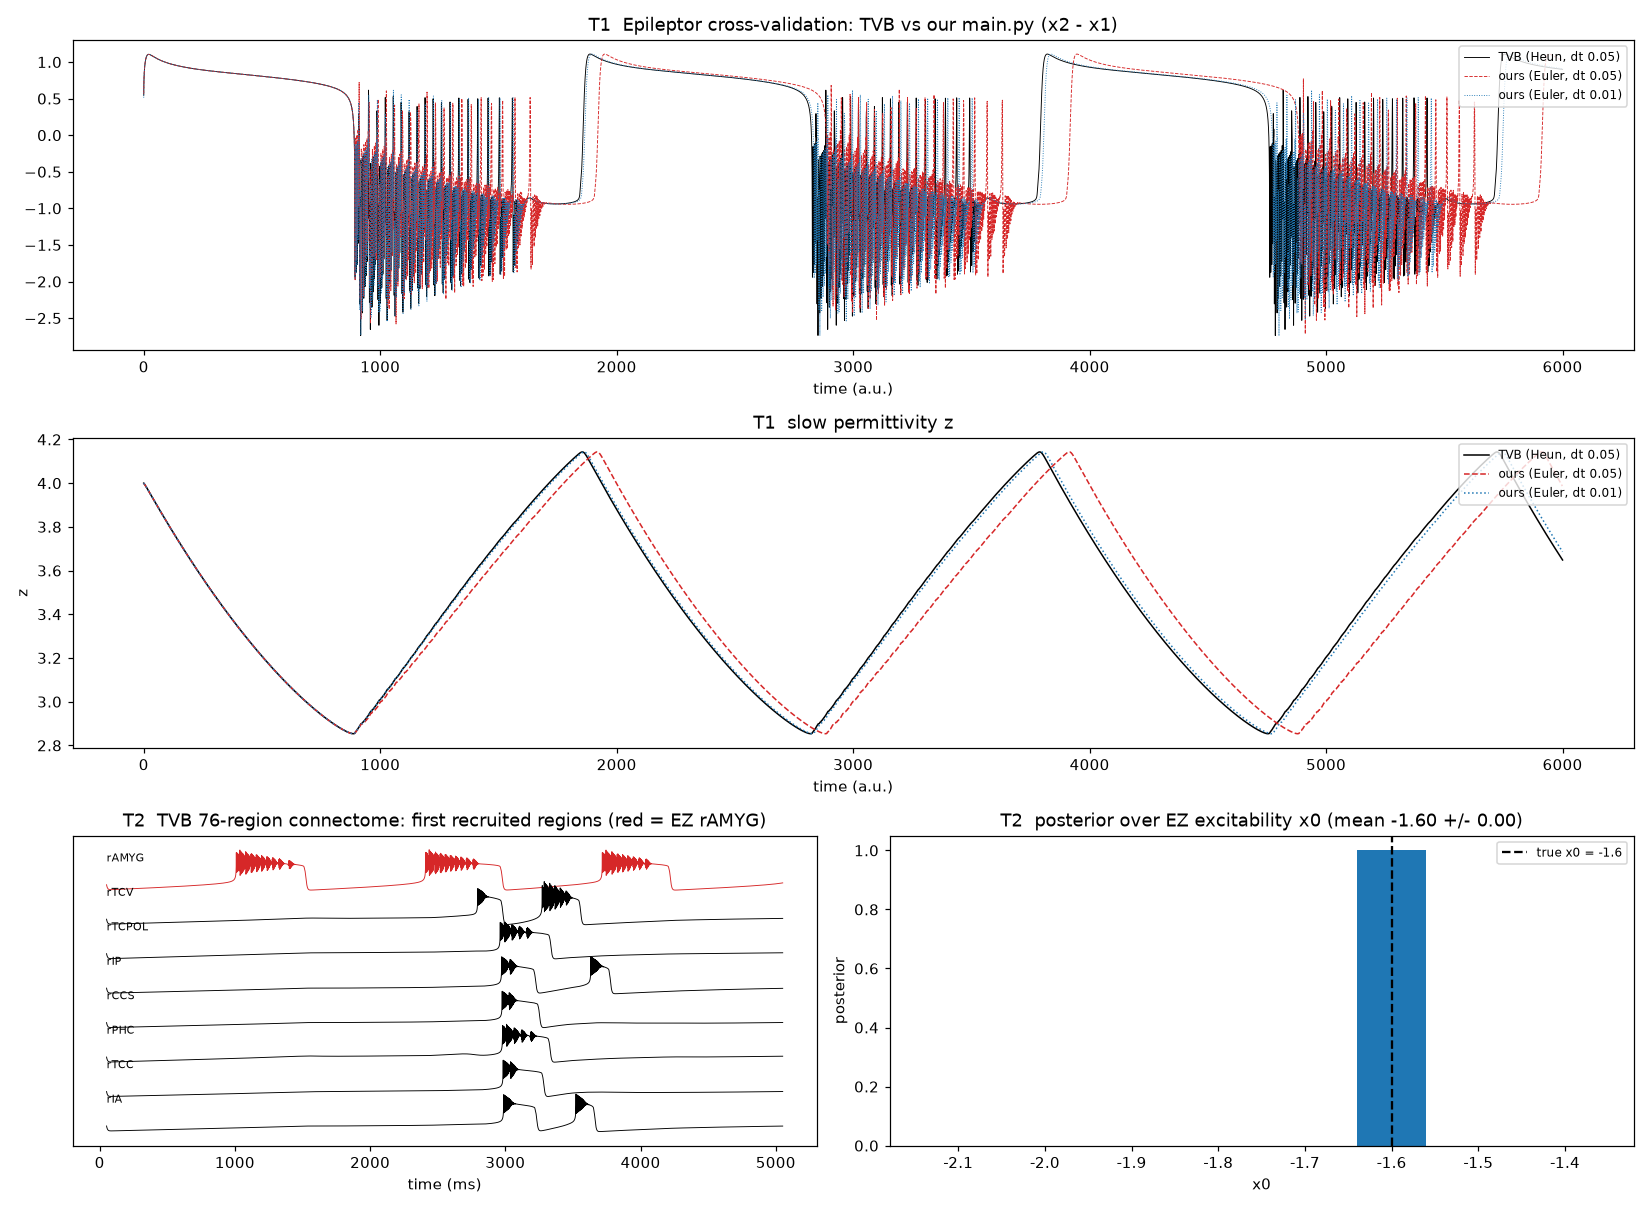
\includegraphics[width=0.85\linewidth]{epilepsy_sim/output/tvb_compare.png}
\caption{TVB cross-validation (T1) and VEP-style inference (T2).}
\end{figure}

\subsection{Head-to-head and conclusions}

Our ionic model is biophysical, local ($\approx$1\,mm\textsuperscript{2}), infers ions in physical units and answers \emph{why} tissue is epileptic; TVB is phenomenological, whole-brain, localises and propagates seizures and answers \emph{where}. They are complementary: TVB would locate the epileptogenic zone, \code{ionic.py} fitted to that region's EEG, TMS-EEG and fNIRS would infer the mechanism (KCC2 vs glia vs clearance), and the ionic pathology could be mapped back onto TVB's $x_0$ (the Epileptor-2 motivation of Chizhov et al.\ 2018). Overall: derived formulas work when their assumptions hold and fail exactly as predicted when they do not (textbook slope $-16$\%, naive DC 2.4$\times$, GHK bias +2.7\,mM, naive fNIRS 22\% amplitude); model-based inference beats single-formula conversion; some variables (adenosine, KCC2) need the full model; and the code is validated twice (Cressman and TVB).

% ============================================================================
\section{Seizure detection on real scalp EEG (CHB-MIT)}
\label{sec:chbmit}

After the theory phase, the first practical question was: how well do temple or ear-level electrodes detect seizures on real EEG, compared with a full cap?

\subsection{Data}

The CHB-MIT Scalp EEG Database (PhysioNet; Open Data Commons Attribution v1.0; Shoeb 2009) contains long-term paediatric recordings at 256\,Hz with bipolar 10--20 montages and clinician-marked seizure onsets and offsets. Two studies were run: a patient-specific study on 3 patients (chb01, chb03, chb05: all seizure recordings plus 6 seizure-free files each; 19 seizures, 36.6\,h), and a general-model study on all subjects (chb01 and chb21 are the same child and were merged, giving 23 subjects; every seizure recording plus 3 seizure-free recordings per subject; 207 recordings, 185 seizures, 297\,h).

\subsection{Detection pipeline}

All steps are causal (usable in real time on a device):
\begin{enumerate}
\item Band-pass 0.5--45\,Hz (4th-order Butterworth); 2\,s windows every 1\,s, each scored at its end.
\item 14 features per channel: line length, log variance, Hjorth mobility and complexity, log band power in $\delta$ (0.5--4), $\theta$ (4--8), $\alpha$ (8--13), $\beta$ (13--30), $\gamma$ (30--45\,Hz), and the five relative band powers.
\item HistGradientBoosting (150 trees, learning rate 0.1, 31 leaves, class-balanced).
\item Causal 5\,s moving average of the probability, alarm on crossing a threshold, then a 60\,s refractory period.
\end{enumerate}
Event metrics: a seizure is detected if an alarm fires between 15\,s before onset and the seizure end; alarms within 60\,s after a seizure are not false alarms; sensitivity, false alarms per 24\,h (FA/day) and latency (alarm minus onset) are reported.

\subsection{Patient-specific study (3 patients, 19 seizures, 36.6 h)}

Montages: the full 18-channel bipolar cap; ``both temples'' (4 channels: T7--FT9, F7--T7, FT10--T8, F8--T8; FT9/FT10 sit just in front of the ears); right temple (FT10--T8, F8--T8); left temple (T7--FT9, F7--T7); right temple single channel (FT10--T8). Evaluation was leave-one-recording-out (each hour tested by a model that never saw it) and, for comparison, cross-patient (train on the other two patients).

\begin{table}[H]
\centering\small
\caption{CHB-MIT, 3 patients, threshold 0.5.}
\label{tab:chb3}
\begin{tabular}{@{}lcccccc@{}}
\toprule
& \multicolumn{3}{c}{Patient-specific} & \multicolumn{3}{c}{Cross-patient} \\
\cmidrule(lr){2-4}\cmidrule(lr){5-7}
Montage & Caught & FA/day & Latency & Caught & FA/day & Latency \\
\midrule
Full cap (18 ch) & 95\% (18/19) & \textbf{5.2} & 4.5 s & 37\% & 273.8 & 3.0 s \\
Both temples (4 ch) & \textbf{100\%} (19/19) & 9.8 & 6.0 s & 63\% & 306.6 & 18.0 s \\
Right temple (2 ch) & 100\% & 36.0 & 5.0 s & 84\% & 205.0 & 12.5 s \\
Left temple (2 ch) & 100\% & 32.1 & 10.0 s & 79\% & 414.0 & 17.0 s \\
Right temple (1 ch) & 100\% & 62.9 & 5.0 s & 100\% & 226.0 & 8.0 s \\
\bottomrule
\end{tabular}
\end{table}

Patient-specific temple montages caught every seizure, with more false alarms than the full cap (9.8 vs 5.2 per day for both temples); one-sided montages produced 3--6$\times$ more false alarms, the first evidence that \emph{both sides} matter. Cross-patient models on only two training patients generalised poorly (200--400 FA/day). With 36.6\,h, one false alarm counts as 0.66/day, so these figures are coarse, and any stricter thresholds chosen after seeing results are optimistic.

\begin{figure}[H]
\centering
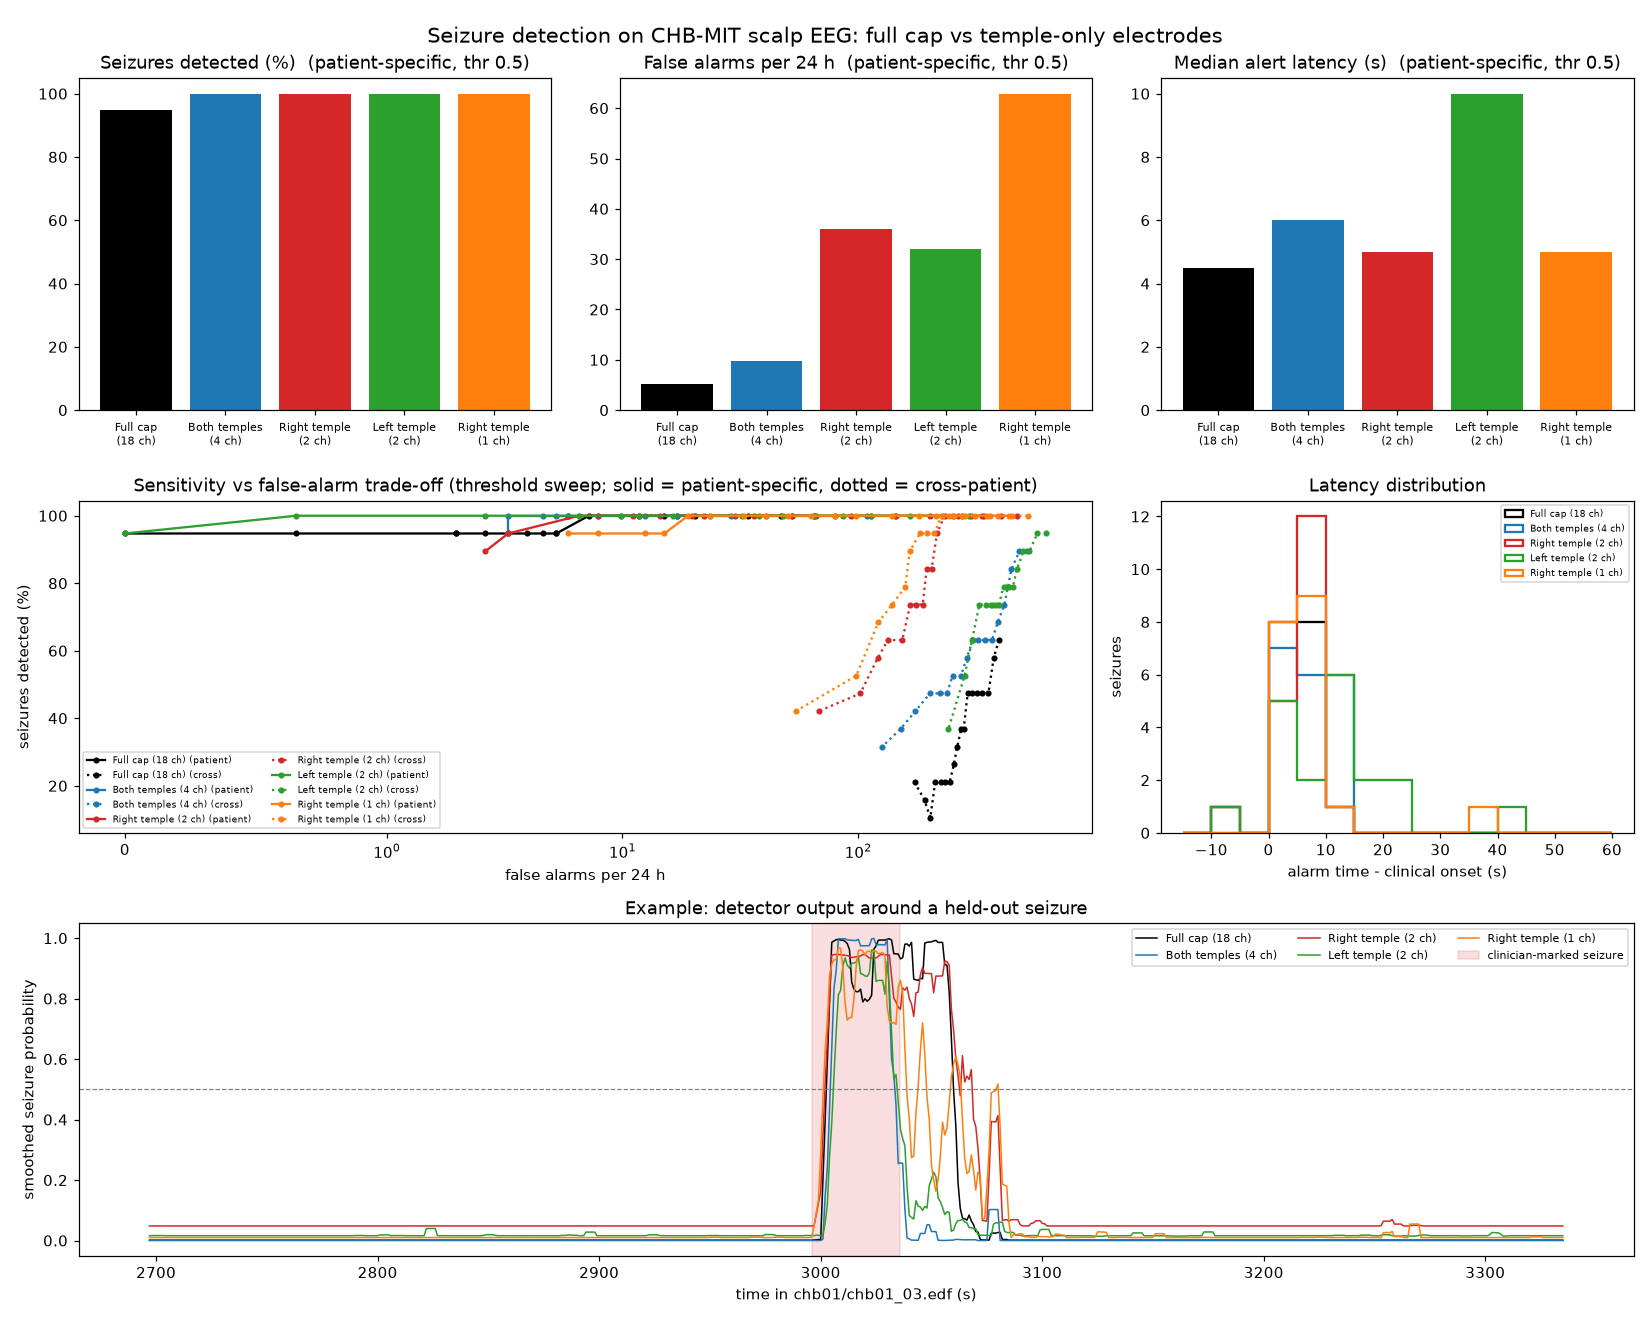
\includegraphics[width=0.8\linewidth]{epilepsy_sim/detect/results/detection.png}
\caption{CHB-MIT patient-specific detection by montage.}
\end{figure}

\subsection{General model (23 subjects, 185 seizures, 207 recordings, 297 h)}

When asked what the cross-patient table meant, and whether a \emph{general} model was possible, a new study was designed (\code{general.py}).

\paragraph{Streaming.} Each EDF was downloaded, converted to features and deleted, keeping disk use near 1\,GB. Files whose montage lacked the 18 standard channels were skipped.

\paragraph{Montages.} Temple (4 ch: F7--T7, T7--P7, F8--T8, T8--P8; FT9/FT10 are not present for every subject); \emph{ear-hook both ears} (2 ch: T7--P7, T8--P8), chosen as the closest standard channels to a ``?''-shaped ear-hook (T7/T8 just above the ear, P7/P8 above and behind it); ear-hook one ear (T8--P8); full cap (18 ch).

\paragraph{Per-person normalisation.} Each feature is z-scored against a causal exponential moving average of the same recording's previous $\approx$10 minutes (EMA over 600 one-second windows, initialised from the first minute), i.e.\ each person is compared with their own recent baseline.

\paragraph{Protocol.} Training pool: all seizure windows plus 5\% of other windows. New-user performance: leave-one-subject-out. Fine-tuning: for subjects with $\ge$3 seizure recordings and at least one seizure-free recording, the first $k$ seizure recordings (k = 1, 2) plus one seizure-free hour were added (patient weight $\times$10) and the model tested on all later recordings, compared with the general model and a patient-only model trained on the same $k$ recordings. A raw-vs-normalised ablation was run on the temple montage.

\begin{table}[H]
\centering\small
\caption{General model, new user (leave-one-subject-out), threshold 0.5.}
\label{tab:general}
\begin{tabular}{@{}lccc@{}}
\toprule
Montage & Caught & FA/day & Median latency \\
\midrule
Temple (4 ch), raw features & 62\% (114/185) & 525 & 6.5 s \\
Temple (4 ch), per-person normalised & 85\% (157/185) & 342 & 6.0 s \\
\textbf{Ear-hook both ears (2 ch)}, normalised & \textbf{88\%} (162/185) & 382 & \textbf{5.0 s} \\
Ear-hook one ear (1 ch), normalised & 83\% (154/185) & 556 & 6.0 s \\
Full cap (18 ch), normalised & 85\% (157/185) & \textbf{229} & 5.0 s \\
\bottomrule
\end{tabular}
\end{table}

\begin{table}[H]
\centering\small
\caption{Fine-tuning on the user's first $k$ seizure recordings (caught / FA per day on later recordings).}
\label{tab:generalft}
\begin{tabular}{@{}llccc@{}}
\toprule
Montage & $k$ & General only & Patient-only & General + fine-tuned \\
\midrule
Temple (4 ch) & 1 & 84\% / 351 & 53\% / 8 & 83\% / 162 \\
 & 2 & 84\% / 361 & 68\% / 16 & \textbf{86\% / 138} \\
Ear-hook both ears (2 ch) & 1 & 86\% / 385 & 54\% / 9 & 83\% / 186 \\
 & 2 & 87\% / 397 & 65\% / 18 & \textbf{86\% / 162} \\
Ear-hook one ear (1 ch) & 1 & 81\% / 547 & 44\% / 13 & 74\% / 241 \\
 & 2 & 81\% / 550 & 66\% / 79 & 80\% / 216 \\
Full cap (18 ch) & 1 & 83\% / 240 & 56\% / 3 & 84\% / 95 \\
 & 2 & 84\% / 246 & 68\% / 6 & \textbf{89\% / 88} \\
\bottomrule
\end{tabular}
\end{table}

At stricter thresholds (chosen after seeing results, hence optimistic), fine-tuned detectors reached $\approx$18--23 FA/day while catching 64\% (ear-hook both ears) to 75\% (full cap) of seizures.

\begin{figure}[H]
\centering
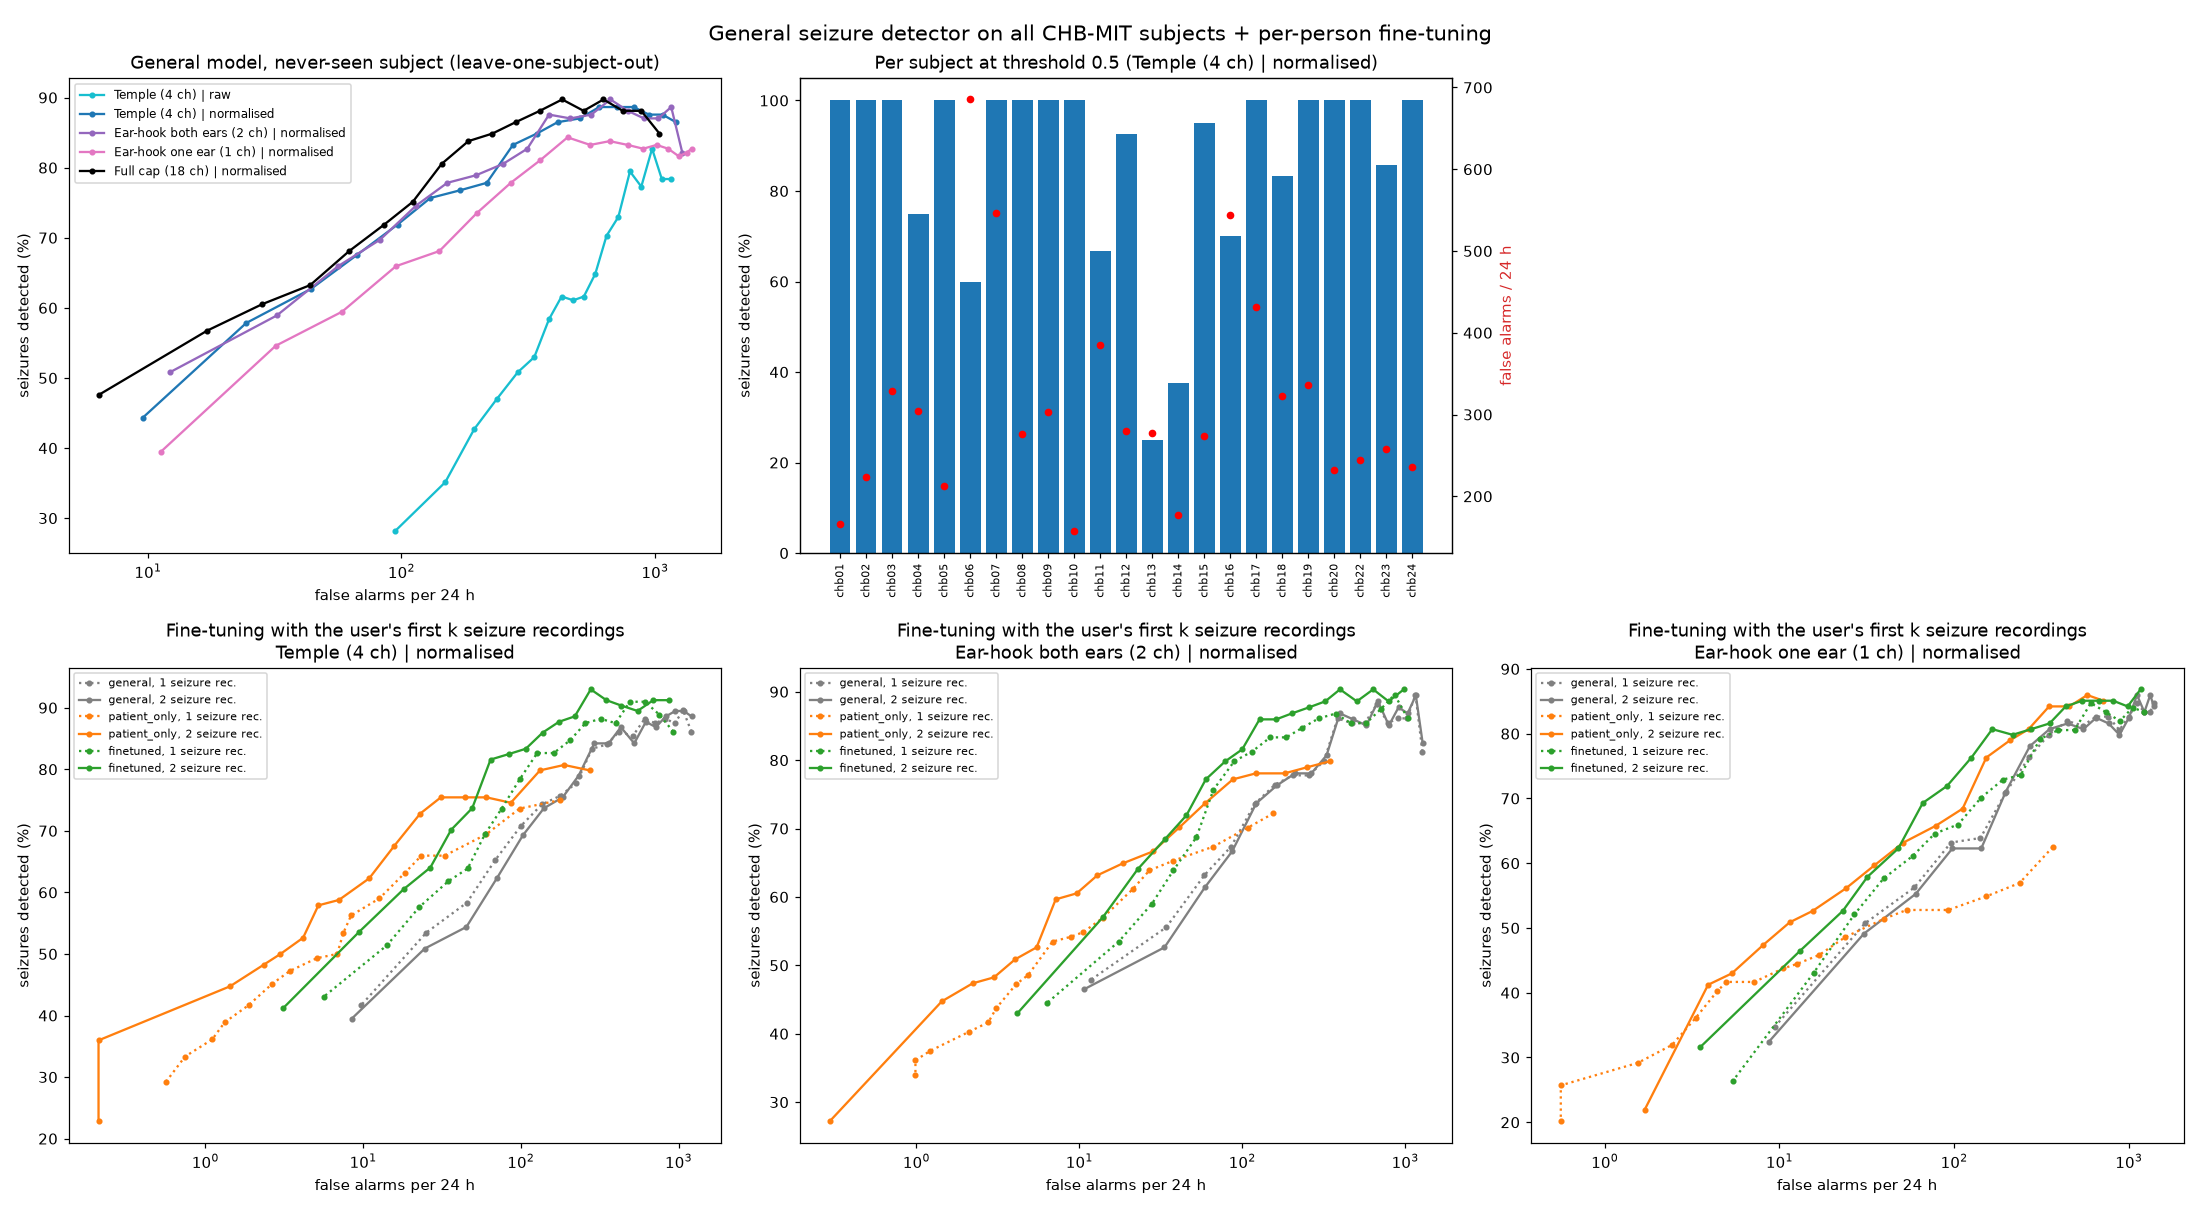
\includegraphics[width=0.95\linewidth]{epilepsy_sim/detect/results_general/general.png}
\caption{General model on all CHB-MIT subjects and personal fine-tuning.}
\end{figure}

\paragraph{Findings.}
\begin{enumerate}
\item Per-person normalisation added 43 detected seizures to the temple montage (62\%$\to$85\%) while reducing false alarms.
\item Fine-tuning on two own seizure recordings cut false alarms by 40--65\% without losing seizures.
\item The two-channel ear-hook matched the four-channel temple montage and caught as many seizures as the 18-channel cap (88\% vs 85\%); the extra channels mainly buy false-alarm rejection ($\approx$2$\times$ fewer).
\item Both ears beat one ear: about 6\% more seizures and 25--30\% fewer false alarms.
\item Patient-only models had few false alarms but missed about a third of seizures; two examples are too few to learn from alone.
\item Absolute false-alarm rates (hundreds per day for new users) were far too high: the decisive motivation for adding body signals.
\end{enumerate}

\subsection{Operational issues and fixes}

PhysioNet downloads ran at $\approx$153\,KB/s, so the AWS open-data mirror was used. File \code{chb02_16+.edf} returned HTTP 404 until its name was URL-encoded; network errors were made non-fatal and retried on the next run. Long runs inside the assistant's session were repeatedly killed by memory-pressure reaping, so heavy jobs were thereafter run by the user in their own terminal, with resumable checkpoints (results saved as soon as each configuration's general stage finished; per-configuration random seeds from a CRC32 of the name). A \code{tqdm.write(flush=...)} keyword crashed a run and was removed. A PNG locked by an image viewer triggered a timestamped fallback file. Phone notifications (ntfy) announced completion, crashes or stopped processes; a small notifier script also served as the requested ``phone call'' feature.

% ============================================================================
\section{The device concept: a ``?''-shaped ear-hook}
\label{sec:device}

Instead of a temple pod, the user proposed an ear device shaped like a question mark, worn on both ears. Its top curve carries dry EEG electrodes above and behind the ear (near T7/T8 and P7/P8), the back stem a mastoid reference, the ear-canal tip in-ear EEG, PPG and temperature, with an optional earlobe PPG, a 6-axis IMU, jaw-muscle (temporalis) EMG and Bluetooth to a phone.

{\footnotesize
\begin{verbatim}
        ___
      /     \   <- top curve: dry EEG electrodes above/behind the ear (~T7/T8, P7/P8)
     |       |
      \      |  <- back stem: mastoid reference electrode, temporalis EMG
       ?     |
       |    /   <- ear-canal tip: in-ear EEG + PPG + SpO2 + temperature
       .   /    <- optional earlobe PPG
   + 6-axis IMU (accelerometer, gyroscope) . Bluetooth to phone . worn on BOTH ears
\end{verbatim}
}

\begin{table}[H]
\centering\small
\caption{Why the ear.}
\begin{tabularx}{\linewidth}{@{}l L@{}}
\toprule
Reason & Evidence \\
\midrule
Over the temporal lobe, the commonest seizure origin in adults & Ear-EEG matched scalp EEG for temporal-lobe seizures (Zibrandtsen 2017) \\
Proven for seizure detection & Behind-the-ear 2-channel wearable caught 98\% of absence seizures (Swinnen 2021) \\
Good PPG site & Earlobe PPG up to 6.3$\times$ better signal than the wrist; in-ear SpO\textsubscript{2} valid 70--100\% \\
Discreet and stable & Looks like a hearing aid or earbud \\
Both ears $>$ one ear & 3--6$\times$ fewer false alarms than one-sided montages (CHB-MIT, Table~\ref{tab:chb3}); +6\% seizures and $-$25--30\% false alarms in the general model \\
\bottomrule
\end{tabularx}
\end{table}

When asked which configuration would be most accurate, the answer from Table~\ref{tab:generalft} was that the full cap with fine-tuning has the fewest false alarms (88/day) but that the two-ear hook catches about as many seizures, and that false alarms should be handled by additional signals (multimodal agreement, artefact sensors, tiered alerts, personal learning, risk forecasting), which led to the body-signal review and the SeizeIT2 study.

% ============================================================================
\section{The Epilepsy Live Lab: an offline interactive visualisation}
\label{sec:livelab}

The user proposed an HTML page with ``a field of glowing orbs of different colours'' fluctuating with the data, plus live graphs. The result, \code{viz/epilepsy_live.html}, is a single self-contained offline page (no libraries, no internet) fed by \code{viz/data.js} ($\approx$3.4\,MB), generated by \code{viz/export_data.py} from the saved ionic simulations, the inference results, the CHB-MIT data and the detector outputs.

\subsection{Layout and panels}

A one-screen, no-scroll grid (first 12$\times$6, later 12$\times$7) holds: the neuron field; live readouts; nine model charts (LFP, firing rate, \Ko{} with the Kalman-filter and naive device estimates, \Cli{} with the inferred value and \EGABA, \Nai{} and pump flux, adenosine, CBF/HbO/HbR, reversal potentials, and a 100-cell $\times$ 20\,s \Ko{} space map); an EEG panel; the detector probability; band powers with line length; and later a row of body sensors. Controls select the tissue (epileptic/healthy), playback speed, pause, and the EEG source. Deep links reproduce any view: \code{?scen=&t=&eeg=&speed=&paused=&type=&walk=&view=&h=&boot=}.

\subsection{The orb field (first version)}

The 100 neurons sat on a ring (excitatory blue-white, inhibitory pink), flashing on spikes; orange particles around each neuron represented its local \Ko; a gold core glow showed \Nai; cyan satellites orbiting each neuron showed \Cli{} loading; a violet haze showed adenosine; glowing blood vessels were coloured by the HbO/HbR balance and pulsed at the heart rate.

\subsection{Real vs model EEG and the virtual ear-EEG forward model}

The first EEG panel showed a 3-minute, 5-channel excerpt of CHB-MIT \code{chb01_03.edf} (2926--3106\,s file time; clinician seizure at 2996--3036\,s), with the trained both-temples detector. The user asked whether model and real EEG were the same source (they were not: separate clocks), and proposed replacing the real recording with ``recordings from the model''. A forward model was therefore written that computes what ear electrodes around the simulated patch would record:
\begin{equation}
\mathrm{ch}_e(t) = g\sum_c w_{ec}\,s_c\,(\mathrm{spikes}_c * \kappa)(t) \;-\; \alpha\cdot51\,\mathrm{mV}\cdot\log_{10}\frac{[\mathrm K]_{o,\mathrm{local}}}{[\mathrm K]_{o,\mathrm{rest}}} \;+\; \eta_{1/f}(t),
\end{equation}
with Gaussian ring-distance weights $w_{ec}$ ($\sigma=20$ cells), signs $s_c=+1$ (excitatory) or $-1.5$ (inhibitory), a synaptic kernel $\kappa(t)=e^{-t/8\,\mathrm{ms}}-e^{-t/2\,\mathrm{ms}}$, a gain $g$ set so the healthy baseline carries $\approx$10\,\uV{} RMS of neural signal (shared between tissues), a glial \Kp{} DC shift reaching the scalp with $\alpha=1$\%, and pink background noise (6\,\uV, half shared across channels; 3\,\uV{} on the DC channel). Four virtual electrodes (V1--V2 right ear, V3--V4 left ear) plus a DC channel were exported at 128\,Hz with the same 14 features as the real detector.

A line-length detector \textbf{failed} on this virtual EEG because the model's ictal event is tonic firing, which band-passed EEG barely separates from interictal bursts. The detector was replaced by a \Kp-DC detector: the causal 1\,s mean of the DC channel below $-150$\,\uV{} (local \Ko{} $\gtrsim$8\,mM) raises an alarm, with a sigmoid probability $1/(1+e^{(\mathrm{DC}+150)/15})$ and a 60\,s refractory period. The threshold was chosen on the model itself and is not independently validated. In epileptic tissue it alarms at $t=11$\,s (1\,s after trigger onset); in healthy tissue it stays silent.

\subsection{Body sensors and EEG-only vs multimodal detection}

To show how body signals affect detection, a body module generates the SeizeIT2 modalities from the simulated seizure. Because the 100-neuron patch models only the onset zone, the spread to autonomic and motor areas uses literature timings (clinical seizure 40\,s from the trigger; ictal HR +53\% in focal seizures, $\approx$+100\% in tonic-clonic). Four seizure types are selectable: focal non-motor, focal motor (hyperkinetic), focal-to-bilateral tonic-clonic, and ``no HR response'' ($\approx$18\% of patients). A 12\,s walk episode can be switched on.

\paragraph{Heart.} A sympathetic drive $s$ follows the clinical seizure with rise/recovery time constants 6/50\,s; walking adds a drive $w$ (8/20\,s). Heart rate on a 10\,Hz grid is $HR = HR_0(1+h_{type}s) + 18w + d$ with $HR_0=68$\,bpm and a slow random drift $d$. Beats are generated with respiratory sinus arrhythmia at 0.25\,Hz whose amplitude (3\,bpm) shrinks with vagal withdrawal $(1-0.8s)$, plus 10\,ms jitter. The ECG is synthesised as Gaussian P, Q, R, S, T waves per beat (ECGSYN-style), with the T wave placed by Bazett $\sqrt{RR}$, baseline wander, noise and muscle contamination.

\paragraph{Muscle and motion.} Shoulder EMG is white noise with an envelope: 5\,\uV{} baseline; arm swing when walking; irregular 45\,\uV{} activity in hyperkinetic seizures; in tonic-clonic seizures a continuous 130\,\uV{} tonic phase (10\,s), then clonic bursts of 120\,ms slowing from 4 to 1\,Hz, then postictal atonia. Accelerometer magnitude shows 1.8\,Hz step impulses when walking, irregular large movements in hyperkinetic seizures, a 9\,Hz tremor in the tonic phase and decaying jerk impulses in the clonic phase.

\paragraph{Walking artefact.} Each step rocks the ear electrodes (biphasic transients) and a slow electrode-pressure drift of $-240$\,\uV{} appears on the DC channel, which deliberately fools the EEG-only \Kp-DC detector.

\paragraph{Fusion rule (illustrative, hand-set).} On a 1\,s grid, $HR_{10}$ is the mean instantaneous HR over the last 10\,s, a causal 1-minute baseline $B$ tracks it, activity $a$ is the 10\,s standard deviation of acceleration, and the heart rate the movement explains is $E = B + \min(20, 150a)$. EMG ratio $r$ is the 4\,s RMS over its causal 2-minute log-baseline. Body evidence is
\begin{equation}
b = \max\!\Big(\sigma\big((HR_{10}-E-12)/2.5\big),\ \sigma\big((r-4)/0.6\big)\Big),
\end{equation}
and the multimodal score multiplies the maximum EEG probability over the last 30\,s by the maximum body evidence over the last 10\,s. An early version looked back 40\,s for body evidence; when a walk followed a seizure, lingering postictal tachycardia combined with the walking artefact produced a false multimodal alarm, so the window was shortened to 10\,s (``current'' body evidence).

\begin{table}[H]
\centering\small
\caption{Live Lab results with the walk episode on.}
\begin{tabular}{@{}lll@{}}
\toprule
Body setting & EEG-only & Multimodal (EEG confirmed by body) \\
\midrule
Focal non-motor & caught +1 s, 1 false alarm (walk) & caught +9 s, 0 false \\
Focal motor & caught +1 s, 1 false & caught +5 s, 0 false \\
Tonic-clonic & caught +1 s, 1 false & caught +6 s, 0 false \\
No HR response & caught +1 s, 1 false & \textbf{missed}, 0 false \\
Healthy tissue & 1 false & 0 false \\
\bottomrule
\end{tabular}
\end{table}

This anticipated, qualitatively, the trade-off later measured on real data: body confirmation removes movement false alarms but costs a few seconds and misses seizures without a body sign. The live score first printed ``MISSED'' before the confirmation window had elapsed; it now shows ``watching\dots'' during a seizure.

\subsection{The 3D neuron plane}

The user asked for something ``more insane'': a plane of neurons fluctuating on the $z$ axis with fixed $x,y$. The 100 neurons were laid out on a 10$\times$10 grid in ring order snaking row by row, so ring neighbours stay plane neighbours. Each neuron's height is its \emph{own} data: local \Ko{} (slow swell), a spike trace (fast jolt), or both (selectable). A surface interpolated between neurons (visual only) is coloured by \Kp{} with a magma palette and depth-sorted; spikes emit ripples; orange \Kp{} ``vapour'' rises in proportion to local \Kp{} excess; \Clm{} satellites orbit; blood vessels run beneath; the view auto-rotates and supports drag, zoom and reset, all in plain canvas 3D projection. Initial renders were too large and blew out to white at the seizure peak; heights, perspective, mote rate and glow were reduced. The original ring remains one click away. Only 100 neurons exist in the simulation; a denser plane would require re-running \code{ionic.py} with more cells.

\subsection{The HUD interface}

Finally the interface was restyled as a ``Stark-lab'' heads-up display: a boot sequence (spinning arc reactor and typed log lines, skippable with \code{?boot=0}); holographic panels with corner brackets, a grid backdrop, scanlines and a sweeping beam; arc-reactor ring gauges for the eight readouts (conic gradients whose cores brighten with the value); glowing chart traces; a targeting reticle over the neuron field whose colour shifts from cyan to red with \Kp{} load and which flashes ``ICTAL THRESHOLD''; a flashing alert badge in ictal phases; and a ``JARVIS'' narration box. Everything stays offline (system fonts only).

\subsection{Bugs fixed in the Live Lab}

JSON serialisation of int64 values failed in the exporter; a CSS class \code{dash} for dashed legend keys clashed with the \code{.dash} grid and was renamed \code{dsh}; a negative \code{requestAnimationFrame} time step produced NaN and was clamped at zero; the multimodal 40\,s look-back and premature ``MISSED'' label were fixed as described; and the headless-browser screenshot job used for checking hung on the endless animation until a hard timeout was used.

% ============================================================================
\section{Multimodal detection on wearable data (SeizeIT2)}
\label{sec:seizeit2}

\subsection{Dataset}

SeizeIT2 (Bhagubai et al.\ 2025; OpenNeuro ds005873 v1.1.0, CC0) was recorded with the Byteflies Sensor Dot in five European epilepsy monitoring units (Leuven, Freiburg, Aachen, Karolinska, Coimbra). It is almost exactly the ear-hook's sensor set.

\begin{table}[H]
\centering\small
\caption{SeizeIT2 as used here.}
\begin{tabularx}{\linewidth}{@{}l L@{}}
\toprule
Patients & 125 with focal epilepsy (51 female; children only from Leuven) \\
Seizures & 883 focal (aware, impaired awareness, focal-to-bilateral tonic-clonic, unclear); mean 58 s (3 s -- 16 min) \\
Recording & 11,626 h in 2,850 runs \\
EEG & 2 behind-the-ear (mastoid) channels, 256 Hz: a same-side channel and a cross-head channel (or two lateral channels in a ``generalized'' montage); montage left/right/generalized in 65/44/16 patients \\
ECG, EMG & 1 chest ECG channel and 1 left-deltoid EMG channel, 256 Hz \\
Motion & Accelerometer and gyroscope on two devices (upper back, chest), 25 Hz \\
Missing & ECG/EMG absent in 46 runs, motion in 299 runs \\
Labels & Clinician-marked onset/offset from video-EEG; type, lateralization, localization, vigilance; ``bckg'' background and ``impd'' epochs \\
\bottomrule
\end{tabularx}
\end{table}

\subsection{Streaming 126 GB through memory}

The dataset is 126\,GB and the laptop had 19\,GB free. The user asked whether training could use the data online without compromising quality: streaming reads exactly the same samples a download would, so it loses no quality. For each run the four EDF files were fetched in parallel from S3 into RAM, decoded by a small built-in EDF reader (header fields: labels, physical and digital ranges, samples per record; int16 data scaled to physical units, EDF-Annotations channel skipped), converted to features, and only the features were saved atomically (1.8\,GB total). Three runs streamed in parallel over 12 connections at 18--25\,MB/s; the job was resumable. The file listing was obtained from the S3 API (2,850 event files downloaded in parallel).

\subsection{Features}

Signals were cut into 4\,s windows every 2\,s (enough heartbeats for HR; manageable for 11,600\,h); a window is ``seizure'' if its centre lies in a marked seizure.

\begin{itemize}
\item \textbf{EEG (2 ch, 28 features):} band-pass 0.5--45\,Hz; per channel line length, log variance, Hjorth mobility and complexity, five log band powers and five relative band powers (Hann-windowed FFT), identical to the CHB-MIT features.
\item \textbf{ECG (8):} R-peaks by a Pan--Tompkins-style detector (5--20\,Hz band-pass, squared derivative, 120\,ms moving average, adaptive threshold at 30\% of the 98th percentile per 10\,s block, 270\,ms refractory), RR intervals kept if 0.27--2.0\,s and within 30\% of a 9-beat running median; features HR over 4, 10 and 30\,s, 30\,s HR rise, RMSSD and SDNN over 30\,s, beat quality (beats found vs expected) and ECG line length.
\item \textbf{EMG (5):} 20--120\,Hz band-pass with a 48--52\,Hz notch; log RMS, line length, zero-crossing rate, fraction of power above 60\,Hz, and 0.5--20\,Hz log power.
\item \textbf{Motion (8):} per device, log standard deviation and line length of acceleration magnitude, fraction of power at 2--8\,Hz (clonic band) and mean gyroscope magnitude.
\end{itemize}

Every feature is z-scored against a causal exponential moving average of the previous $\approx$10\,min of the same recording (EMA over 300 two-second windows); absolute HR and beat quality are also kept. Missing sensors stay NaN and are routed separately by the trees, so no patient is dropped.

\subsection{Models and evaluation}

HistGradientBoosting (150 trees, class-balanced) trained on all seizure windows plus 3\% of others; patient-wise 5-fold cross-validation balanced by seizure count (every patient scored by a model that never saw them); probability smoothed over 3 windows (6\,s), threshold, 60\,s refractory; a seizure is caught if an alarm fires from 15\,s before onset to its end, other alarms are false except within 60\,s after a seizure; thresholds swept from 0.05 to 0.99.

The fair comparison is false alarms at \emph{matched sensitivity}: the fewest false alarms at any threshold catching at least X\%. \textbf{A bug was caught here}: the first summary interpolated false alarms along the sensitivity curve, but sensitivity is not monotonic in the threshold (at low thresholds a false alarm just before a seizure starts the refractory period and blocks the true alarm), which produced nonsense (EEG-only apparently 1,300\,\FAd{} at 60\%); it was replaced by the minimum over thresholds.

Two kinds of numbers are reported. \emph{Calibrated} numbers fix the threshold in advance on tuning data and score later data (what a device would experience). \emph{Best-along-the-curve} numbers sweep the threshold over the test data and report the best point within a budget; they compare setups fairly but are slightly optimistic for deployment. For the one-stage general model the two agree closely (14\%/25\% at $\le$1/$\le$5 per day both ways).

\subsection{Main results (125 patients, 883 seizures)}

\begin{table}[H]
\centering\small
\caption{False alarms per 24 h at matched sensitivity (lower is better).}
\label{tab:sz2main}
\begin{tabular}{@{}lcccc@{}}
\toprule
Setup & 50\% caught & 60\% & 70\% & 80\% \\
\midrule
EEG only (ear) & 103.7 & 161.7 & 294.4 & not reached \\
ECG only & 132.6 & 225.6 & 378.2 & 677.8 \\
Body only (ECG+EMG+motion) & 116.3 & 193.5 & 283.8 & 583.1 \\
\textbf{EEG + ECG} & \textbf{85.5} ($-18$\%) & \textbf{122.8} ($-24$\%) & \textbf{204.0} ($-31$\%) & \textbf{459.2} \\
EEG + ECG + EMG + motion & 75.4 ($-27$\%) & 139.3 ($-14$\%) & 211.7 ($-28$\%) & 539.9 \\
\bottomrule
\end{tabular}
\end{table}

\begin{table}[H]
\centering\small
\caption{Seizures caught within a daily false-alarm budget, and at the default threshold 0.5.}
\begin{tabular}{@{}lccccc|ccc@{}}
\toprule
Setup & $\le$5 & $\le$20 & $\le$50 & $\le$100 & $\le$200 & Caught @0.5 & FA/day & Latency \\
\midrule
EEG only & 14\% & 23\% & 23\% & 42\% & 62\% & 79.4\% & 608 & 6 s \\
ECG only & 16\% & 29\% & 29\% & 48\% & 60\% & 74.0\% & 438 & 7 s \\
Body only & 16\% & 28\% & 42\% & 50\% & 64\% & 75.4\% & 386 & 8 s \\
\textbf{EEG + ECG} & \textbf{21\%} & \textbf{35\%} & 35\% & \textbf{57\%} & 66\% & 78.7\% & \textbf{399} & 7 s \\
All four & 20\% & 34\% & \textbf{45\%} & 53\% & \textbf{68\%} & 78.3\% & 348 & 7 s \\
\bottomrule
\end{tabular}
\end{table}

Per patient, the median false-alarm rate fell from 618 (IQR 533--686) with EEG to 373 (329--440) with EEG + ECG and 342 (299--400) with all four; EEG + ECG had fewer false alarms than EEG alone in \textbf{115/125} patients (all four: 120/125), while detections per patient barely changed (more in 16, fewer in 21). Heart rate is the add-on that pays; for focal seizures the heart alone rivals the ear EEG under strict budgets; EMG and motion as direct features give no consistent gain for these mostly non-convulsive seizures. Two interim snapshots taken while streaming (48 patients: $-7$\% to $-20$\%; 78 patients: $-21$\% to $-44$\%) converged to the final $-18$\% to $-31$\%.

\begin{figure}[H]
\centering
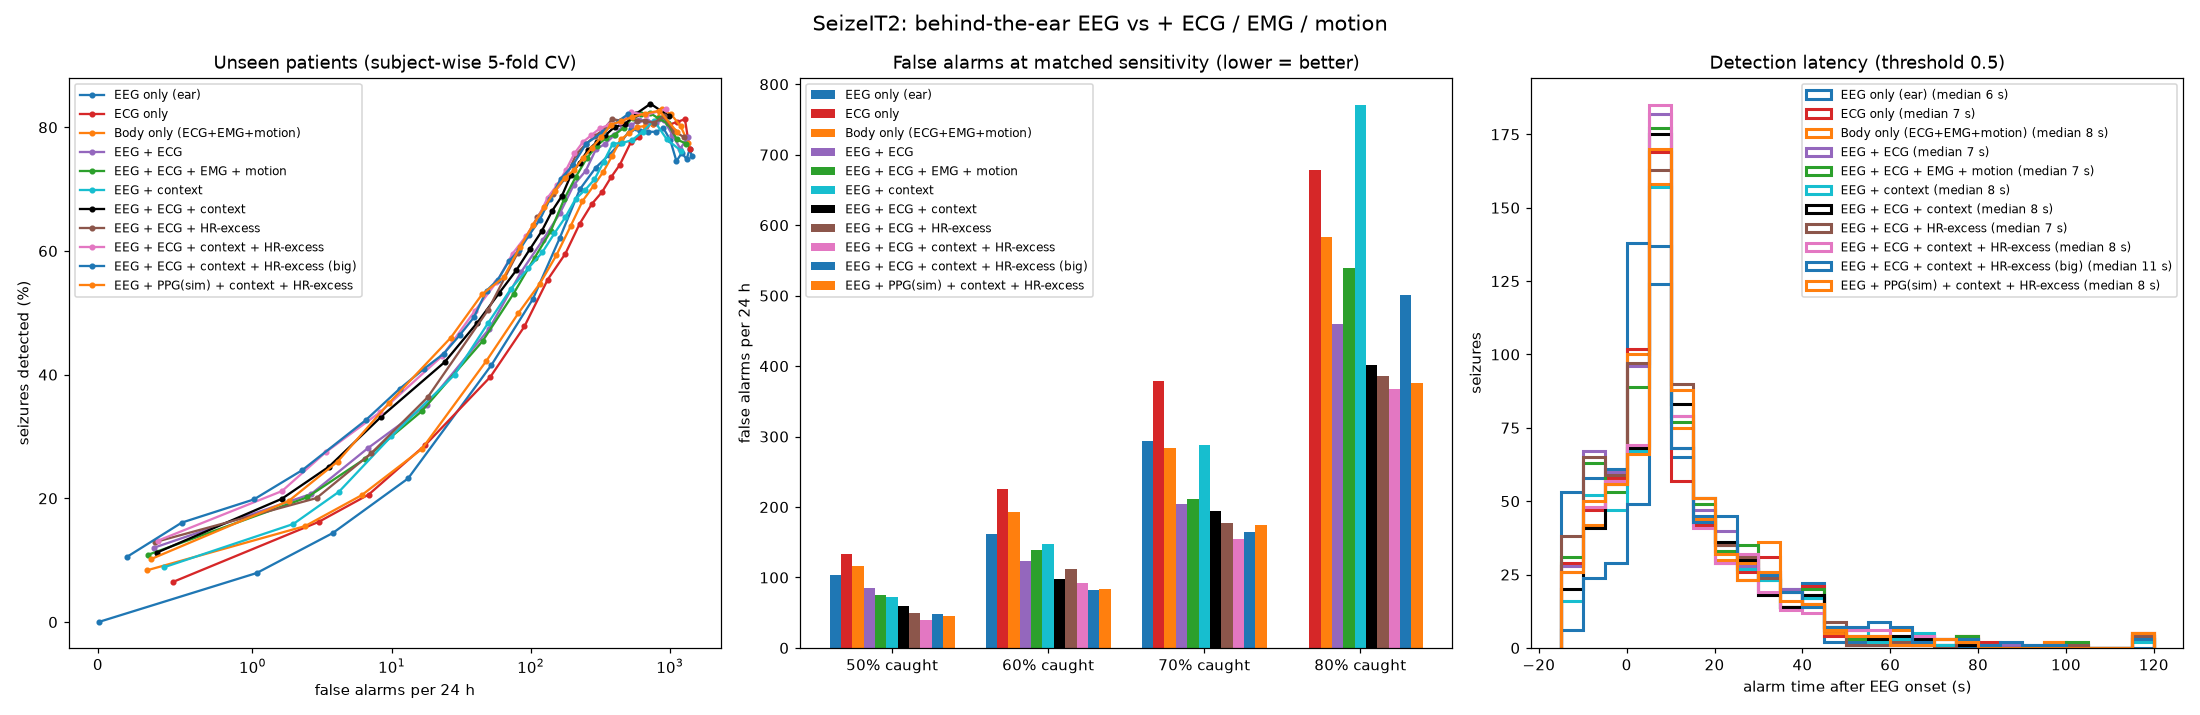
\includegraphics[width=\linewidth]{epilepsy_sim/detect/results_seizeit2/seizeit2.png}
\caption{SeizeIT2: sensitivity vs false alarms, false alarms at matched sensitivity, and latency for all setups (including the later context and HR-excess setups).}
\end{figure}

\subsection{Personal fine-tuning and sustained-alarm rules}

Chronological split per patient: tune on everything up to 10\,min after the $k$-th seizure, test only on later data (71 patients with $k=2$, 649 test seizures; 97 patients with $k=1$, 751). The fine-tuned model adds the patient's tuning windows ($\times$10) to the general model's training data. Three alarm rules were compared: 6\,s smoothing, 10\,s and 20\,s sustained above threshold. A vectorised event scorer was verified identical to the reference scorer on synthetic records before use.

\begin{table}[H]
\centering\small
\caption{Fine-tuning on 2 own seizures (71 patients): FA/day at matched sensitivity and caught within budgets (6 s rule).}
\begin{tabular}{@{}lccccccc@{}}
\toprule
Setup & 40\% & 50\% & 60\% & 70\% & $\le$1/d & $\le$5/d & $\le$20/d \\
\midrule
EEG, general & 100.8 & 157.9 & 221.3 & 289.0 & 0\% & 11\% & 20\% \\
EEG, fine-tuned & 61.5 & 91.6 & 127.9 & 217.1 & 8\% & 15\% & 28\% \\
EEG+ECG, general & 52.4 & 88.7 & 168.0 & 254.7 & 10\% & 18\% & 32\% \\
\textbf{EEG+ECG, fine-tuned} & \textbf{40.5} & \textbf{60.5} & \textbf{107.2} & \textbf{192.5} & \textbf{14\%} & \textbf{21\%} & 27\% \\
\bottomrule
\end{tabular}
\end{table}

ECG ($-44$\% at 50\%) and fine-tuning ($-42$\%) add up ($-62$\% together, close to the $-67$\% expected for independent effects), with unchanged delay. With one tuning seizure, EEG-only tuning was inconsistent (better at 40\%, worse at 60\% and under strict budgets: overfitting to one event), whereas with ECG even one seizure helped ($-16$\% to $-45$\%). Sustained rules helped only at low sensitivity, were worse at 60--70\% caught and added 3--7\,s of delay; 6\,s smoothing was kept.

\subsection{Personal alarm thresholds}

For each budget (0.5--200 \FAd), a personal threshold was the lowest threshold whose false alarms on the patient's own tuning data stayed within budget (fallback to shared for $<$6\,h of tuning data: 12 of 71; median tuning 23\,h); the shared threshold used the same rule on pooled tuning data. Personal thresholds gave no meaningful gain (at most +2--4 points at loose budgets, overshooting their budget, never reaching $\le$1/day): per-person baseline normalisation already puts everyone on a common scale (at 5/day, personal thresholds IQR 0.956--0.971 vs shared 0.971). The general model's shared threshold was \emph{predictable}: budgets of 1/5/20 on tuning data gave 1.4/5.2/20.2 \FAd{} later (EEG+ECG). Fine-tuned models calibrated on their own training data were $\approx$10$\times$ optimistic (0.5--1/day became 10--18/day, later 30--37/day for the richest model); calibration needs held-out data.

\subsection{Why do the false alarms happen?}

All analyses used cached outputs (general model, shared threshold, 71 patients). A \textbf{mistake was caught}: the ``impd'' annotation was first assumed to mean interictal epileptiform discharges; the dataset's \code{events.json} defines it as an \emph{impedance control check} (likely artefactual). Such epochs explained $<$1\% of false alarms (2--5$\times$ chance; 0.19\% of time). False alarms were not hidden seizures (7--10\% within 1--30\,min of a seizure vs 8.9\% of time). They were concentrated: at 5/day the worst 10\% of patients produced 47\% (EEG) and 32\% (EEG+ECG) of them, the worst 25\% 77\% and 59\%; the median patient had 1.4 and 4.0/day. Of 22 patient traits, only \textbf{ear-EEG amplitude instability} (IQR of log-variance) survived Bonferroni correction ($\rho=0.49$, $p=1\times10^{-5}$; 2.10 vs 1.18); no link was found with missing sensors, seizure type, number of seizures, electrode side, sex, recording fragmentation or ECG quality (age is not available). At the moment of a false alarm (EEG+ECG, 3,655 false alarms vs 267 detections) the signals looked like seizures: heart rate 103 vs 110\,bpm (normal 73), a 30\,s HR rise of +20 vs +22, raised movement, EEG power and shoulder EMG: physiological look-alikes (getting up, arousals). EEG-only false alarms instead showed muscle/movement in the EEG (gamma share 0.06$\to$0.13) with a calm heart, which is why ECG removes them. Each patient's tuning-period false-alarm rate predicted their later rate ($\rho$ = 0.56--0.83), flagging 73--81\% of the worst quartile.

\subsection{Long context}

For key features (EEG line length, log variance, $\delta$ and $\theta$ shares; HR, RMSSD, SDNN, beat quality) the model received causal EMAs over 15\,s, 1\,min and 5\,min, fast-minus-slow differences, the 1-min running maximum, and heart features against a 30-min baseline, each context setup training on exactly the same windows as its twin (shared random seed). Causality was verified by altering future data and checking that past features were unchanged.

\begin{table}[H]
\centering\small
\caption{Context and HR-excess setups (125 patients, general model).}
\label{tab:ctx}
\begin{tabular}{@{}lccccccc@{}}
\toprule
Setup & 50\% & 60\% & 70\% & 80\% & $\le$5/d & $\le$50/d & $\le$200/d \\
\midrule
Ear EEG only & 103.7 & 161.7 & 294.4 & -- & 14\% & 23\% & 62\% \\
EEG + context & 72.2 & 148.2 & 287.7 & 770.6 & 21\% & 48\% & 65\% \\
EEG + ECG & 85.5 & 122.8 & 204.0 & 459.2 & 21\% & 35\% & 66\% \\
EEG + ECG + context & 59.5 & 98.5 & 194.6 & 401.8 & 25\% & 48\% & 72\% \\
EEG + ECG + HR-excess & 49.2 & 111.7 & 177.7 & 385.8 & 20\% & 50\% & 72\% \\
\textbf{EEG + ECG + context + HR-excess} & \textbf{39.6} & \textbf{92.5} & \textbf{154.9} & \textbf{368.0} & \textbf{28\%} & \textbf{50\%} & \textbf{73\%} \\
same, big model (\S\ref{sec:big}) & 48.2 & 82.8 & 165.0 & 500.6 & 25\% & 54\% & 72\% \\
EEG + PPG(sim) + context + HR-excess & 44.8 & 83.5 & 175.2 & 376.5 & 26\% & 53\% & -- \\
\bottomrule
\end{tabular}
\end{table}

\subsection{Heart rate not explained by movement (HR-excess)}

Per recording, a causal running linear fit of heart rate on activity predicts the heart rate the current movement explains. With $A_t$ the 15\,s EMA of the larger of the two log-acceleration features and $H_t$ the 10\,s heart rate, running EMAs with 30\,min memory of $A$, $H$, $A^2$ and $AH$ (using only past values) give
\begin{equation}
b_t = \mathrm{clip}\!\left(\frac{\overline{AH}_{t-1}-\bar A_{t-1}\bar H_{t-1}}{\max(\overline{A^2}_{t-1}-\bar A^2_{t-1},0.05)},0,30\right),\qquad
\hat H_t = \bar H_{t-1} + b_t(A_t - \bar A_{t-1}),
\end{equation}
and four features: $H_t-\hat H_t$ (HR excess), its 1\,min EMA, $A_t$, and the 30\,s rise not explained by activity, $(H_t-H_{t-30s}) - b_t(A_t-A_{t-30s})$. A univariate pre-check suggested little value (AUC 0.62 vs 0.61 for raw HR in separating false alarms from detections), yet in the full model HR-excess cut false alarms by 42\% at 50\% caught and, with context, gave the best general model (Table~\ref{tab:ctx}): $-62$/$-43$/$-47$\% at 50/60/70\% caught vs ear EEG alone and 28\% caught at $\le$5/day. \textbf{Lesson: a weak single-feature pre-check does not predict a feature's value in combination.}

\subsection{Benchmarks on SeizeIT2}

\begin{table}[H]
\centering\small
\caption{Published SeizeIT2 results vs ours at similar false-alarm rates (protocols differ; order-of-magnitude comparison).}
\begin{tabularx}{\linewidth}{@{}L l l L@{}}
\toprule
Published & Caught & FA/day & Ours \\
\midrule
Dataset paper, SVM, bte-EEG (29 held-out patients) & 71.1\% & 264 (11.0/h) & EEG only 62\% at $\le$200; EEG+ECG+context 72\% at $\le$200 \\
Dataset paper, ChronoNet & 84.2\% & 2,412 & EEG+ECG+context 80\% at 402 \\
ECG Matrix Profile, FAR-optimised (Reintjes 2025) & 19.6\% & $<$48 & ECG only 29\% at $\le$20 \\
ECG TimeVQVAE-AD, FAR-optimised & 36.9\% & 206 & ECG only 60\% at $\le$200 \\
ECG TimeVQVAE-AD, sensitivity-optimised & 82.8\% & 627 & EEG+ECG+context 80\% at 402 \\
ECG Matrix Profile, responders only & 70.7\% & $\approx$46 & EEG+ECG fine-tuned, responders 81\% at $\le$50 \\
\bottomrule
\end{tabularx}
\end{table}

No published SeizeIT2 result approaches 1 \FAd. The 69\% at 0.49 \FAd{} of Vandecasteele et al.\ (2020) used the earlier SeizeIT1 hospital dataset, a 3-channel setup, patient-specific models and only seizures visible on behind-the-ear EEG; the SeizeIT2 paper calls its own wearable results ``sub par''. Real devices keep false alarms low mainly by targeting convulsive seizures (Embrace, NightWatch), night-only use, personal tuning, user cancellation and better electrodes.

\subsection{Heart responders}

A responder is a patient whose heart rate rose by $>$50\,bpm (max 10\,s HR from onset to 60\,s after end minus the 5-min pre-onset median) in at least one of their first two seizures, a definition a device could apply; 23 of 69 patients with ECG are responders.

\begin{table}[H]
\centering\small
\caption{Responders vs non-responders (71 patients, later data; caught within budgets).}
\begin{tabular}{@{}llccc@{}}
\toprule
Model & Group & $\le$1/day & $\le$5/day & $\le$20/day \\
\midrule
EEG only, general & responders / non-resp. & 10\% / 2\% & 21\% / 7\% & 44\% / 16\% \\
EEG+ECG, general & responders / non-resp. & 25\% / 6\% & 46\% / 10\% & 68\% / 18\% \\
EEG+ECG, fine-tuned & responders / non-resp. & 30\% / 7\% & 50\% / 15\% & 72\% / 24\% \\
Best (ctx+HRx), general & responders / non-resp. & 31\% / 7\% & 55\% / 14\% & 74\% / 23\% \\
Best (ctx+HRx), fine-tuned & responders / non-resp. & \textbf{33\%} / 8\% & \textbf{60\%} / 16\% & \textbf{75\%} / 27\% \\
PPG(sim), fine-tuned & responders / non-resp. & 28\% / 8\% & 54\% / 14\% & 69\% / 26\% \\
\bottomrule
\end{tabular}
\end{table}

\subsection{More data and a bigger model}
\label{sec:big}

With 8\% instead of 3\% of non-seizure windows (the 3\% pool a subset of the 8\% one), 400 trees at learning rate 0.05 and 63 leaves, results were mixed (Table~\ref{tab:ctx}) at 3$\times$ the compute: model capacity and training-set size are not the bottleneck; information is.

\subsection{Two-stage detection and a personal alarm verifier}

Stage 1 (best general model, out-of-fold outputs) raises candidates at 0.5 or 0.7 with a 10\,s candidate refractory. A second HistGradientBoosting model (200 trees, 15 leaves) verifies each candidate at 0 or 10\,s after the trigger using the probability's shape (peak, mean, fraction above 0.8 and 0.95, current value), recent noisiness (candidates in the last 10\,min and hour, 5\,min mean probability) and changes vs the 5\,min before in HR, HR slope, RMSSD, beat quality, EEG log variance, line length, gamma and delta shares, EMG and movement, plus HR-excess features; the 60\,s refractory applies only to accepted alarms. It was trained with patient-wise folds and scored on held-out patients' later data. \textbf{A bug was caught}: the first run grouped alarms per patient although each recording's clock starts at 0, so an alarm in one recording was counted in all others; a debug check (ranking by stage-1 peak lost half the seizures) exposed it and scoring was fixed per recording (``accept all'' then reproduced stage 1: 49\% at 79 \FAd{} on the debug subset). The personal verifier additionally trains on the patient's own tuning-period candidates (weighted $\times$20), which are out-of-sample for stage 1.

\begin{table}[H]
\centering\small
\caption{Two-stage results (candidates at 0.5, decision +10 s; 71 patients, later data).}
\setlength{\tabcolsep}{4pt}
\begin{tabular}{@{}lccccc@{}}
\toprule
Setup & $\le$1/d & $\le$2/d & $\le$5/d & $\le$20/d & $\le$50/d \\
\midrule
One stage (general), all & 14\% & -- & 25\% & 36\% & 47\% \\
Two stage, general verifier, all & 15\% & 18\% & 25\% & 38\% & 54\% \\
Two stage, general + quality features & 14\% & 17\% & 26\% & 39\% & 54\% \\
\textbf{Two stage, personal verifier ($\times$20), all} & \textbf{19\%} & \textbf{22\%} & \textbf{30\%} & \textbf{45\%} & \textbf{60\%} \\
Personal verifier $\times$5 / $\times$50, all & 18\% / 19\% & 22\% / 23\% & 29\% / 30\% & 43\% / 46\% & 57\% / 61\% \\
Personal verifier + quality features, all & 19\% & 23\% & 31\% & 45\% & 61\% \\
\textbf{Personal verifier, responders} & \textbf{39\%} & \textbf{47\%} & \textbf{64\%} & \textbf{77\%} & \textbf{85\%} \\
Personal verifier, non-responders & 11\% & 14\% & 17\% & 32\% & 51\% \\
\bottomrule
\end{tabular}
\end{table}

The personal verifier gave the largest strict-budget gain of anything tried, saturating at weights $\times$20--50. Ear-EEG signal-quality features (5-min log-variance instability per channel, fraction of artefact bursts $>$3 above a 30-min median, channel-balance shift) added nothing: electrode instability is a per-patient hardware property that personalisation already absorbs.

\subsection{The ceiling}

The peak smoothed stage-1 probability during each later seizure shows why performance plateaus: 25\% of all seizures (31\% of non-responders') never exceed 0.5 and only 30\% ever reach 0.95 (responders: 65\% exceed 0.95). No alarm logic can recover seizures the detector barely sees; the remaining gap is a signal problem.

\subsection{Which seizures are caught}

At shared thresholds calibrated in advance (best general model, 649 later seizures): focal-to-bilateral tonic-clonic \textbf{100\%} at $\le$5 and $\le$20 \FAd{} (22 seizures; 95\% even with ear EEG alone); focal motor 30\%/44\%; focal aware non-motor 17\%/29\%; focal impaired-awareness non-motor 14\%/26\%; seizures $<$30\,s \textbf{4\%}/13\% (349 seizures, over half of all, 40\% never above 0.5); 30--90\,s 40\%/59\%; $>$90\,s 62\%/78\%; temporal lobe 43\%/54\% vs extratemporal 19\%/33\%; both-ear (generalized) montage 42\%/55\%; same-side 33\%/51\%; awake 28\%/41\% vs asleep 22\%/36\%.

\subsection{Simulated in-ear PPG}

Chest-ECG features were degraded to in-ear PPG quality from the literature: at rest a slowly varying (30\,s) error with bias +0.78\,bpm and SD 2.54\,bpm (in-ear PPG vs ECG, 97 patients, 2,048\,h); $\pm$15\% relative error during movement; 10\% of resting and 50\% of moving windows lost; RMSSD $\pm$30\% and SDNN $\pm$9\% relative error; beat quality lowered; ECG waveform features removed. On a sample recording the simulated PPG differed from ECG by 2.7\,bpm (bias +0.9), with 16\% of windows lost. \textbf{A crash was caught}: the all-NaN ECG-waveform column broke histogram binning (``window shape cannot be larger than input array shape''); the column is now dropped for PPG. Results: general model within noise of ECG (Table~\ref{tab:ctx}); fine-tuned 13/25/37\% vs 15/27/41\% at $\le$1/5/20 \FAd; responders 28/54/69\% vs 33/60/75\%; calibrated general 11/22/37\% at 0.7/4.1/18.7 \FAd{} (ECG: 14/25/38\% at 1.0/4.3/20.2). PPG keeps most of the benefit because detection relies on heart-rate \emph{changes}, which PPG measures well.

\subsection{Deep learning on the raw ear EEG (in progress)}

To test whether raw waveforms carry information that hand-made features miss, \code{cnn.py} streams the EEG again (47.6\,GB), band-passes 0.5--14\,Hz, downsamples to 32\,Hz and stores int16 (0.1\,\uV{} steps, $\approx$5.4\,GB), then trains a small 1D CNN (four conv-BN-ReLU blocks, 16--64 channels, global mean and max pooling, 39k parameters) on 16\,s of 2-channel EEG ending at each 2-s decision point, with the same patient folds, amplitude augmentation and positive-class weighting; its out-of-fold output will be evaluated alone and stacked into the best feature model. CPU PyTorch was added as an optional extra through an \emph{explicit} package index (a first attempt made the resolver look for all packages in the PyTorch index and failed). The stream was slow (0.3--0.7\,MB/s per stream on campus Wi-Fi), and 572 of 805 attempts failed while the college Wi-Fi's captive portal intercepted TLS (``self-signed certificate in certificate chain'') and DNS failed; certificate verification was deliberately \emph{not} disabled, the user logged into the portal, and the resumable stream continued with a disk-space guard (stop below 1.5\,GB free). Results are pending at the time of writing.

% ============================================================================
\section{Discussion}
\label{sec:discussion}

\subsection{What the evidence says, end to end}

\begin{enumerate}
\item \textbf{Temple alone cannot detect seizures.} It measures scalp optical signals over a non-brain artery.
\item \textbf{Seizure chemistry can be simulated and, in principle, inferred.} The ionic model reproduces the known ionic and haemodynamic hallmarks and is validated against Cressman 2009; inference formulas work only when their assumptions hold, and model-based inference beats single-formula conversions. Our Epileptor matches TVB.
\item \textbf{Ear-level EEG sees most seizures but raises too many false alarms on its own.} On CHB-MIT, two ear-position channels matched an 18-channel cap for new users (88\% vs 85\%) with $\approx$2$\times$ the false alarms; per-person normalisation and personal fine-tuning each helped substantially.
\item \textbf{The heart is the body signal that pays.} On SeizeIT2, ECG cut false alarms by 18--44\% at matched sensitivity for 115/125 patients; simulated in-ear PPG keeps most of that benefit.
\item \textbf{Movement matters through the heart, and minutes matter more than seconds.} Heart rate not explained by movement plus 15\,s--5\,min context reduced false alarms by up to 62\% vs ear EEG alone.
\item \textbf{False alarms are personal.} A quarter of users produce most of them; the one linked trait is unstable ear-EEG amplitude (electrode fit); they are predictable from the first days of wear; a personal alarm verifier that learns each user's false alarms is the single most effective strict-budget tool.
\item \textbf{The dangerous seizures are caught.} All focal-to-bilateral tonic-clonic seizures were caught at $\le$5 \FAd.
\item \textbf{The ceiling is the signal.} Short focal seizures ($<$30\,s, over half of all) are nearly invisible to two mastoid channels; a quarter of seizures never raise the detector above 0.5. Better alarm logic cannot close this gap; hardware (contact quality, more or better-placed electrodes) must.
\end{enumerate}

\subsection{Implications for the device (``Prototype 1'')}

The evidence defines a concrete device architecture: bilateral ear-EEG, in-ear PPG, a head IMU and a phone; features computed over a rolling few-minute history; a general model at first use; personal fine-tuning after about two confirmed seizures; a personal alarm verifier; responder-dependent modes (alarm mode for heart responders, with 39\% of seizures caught at $\le$1 \FAd{} and 64\% at $\le$5; a log-only seizure diary for non-responders); a signal-quality gate with a ``reseat'' prompt; user cancellation of alarms (a phase-3 ECG study cancelled all its false alarms this way); and SUDEP-relevant safety alarms (tonic-clonic seizures, bradycardia, desaturation).

Arguments \emph{against} building it now as an alarm: overall performance at $\le$1 \FAd{} (19\%) is not good enough for most users; all numbers come from SeizeIT2's stick-on mastoid electrodes, chest ECG and hospital conditions, while dry ear electrodes in daily life will be worse; electrode fit, the main false-alarm driver, is unmeasured for our own hardware; PPG results are simulated; and a seizure alarm is a regulated medical device whose misses create false reassurance. Arguments \emph{for} building it as a research recording and diary device: only hardware can answer the largest open questions (dry-electrode signal quality, real in-ear PPG while walking, chewing and sleeping); tonic-clonic seizures are already caught; objective seizure counts are clinically valuable because patients under-report; all components exist off the shelf and the software pipeline is ready. The recommendation is to build it first as a recording and seizure-diary device, validated in phases (bench, self-wear by healthy volunteers, then an epilepsy-monitoring-unit partnership with ethics approval), and to enable alarms only when device-specific data support them.

\subsection{Limitations}

\begin{itemize}
\item \textbf{Simulation:} ictal events are not self-sustaining at the default pump setting; the network is small, 1-D, single-type per population, with simplified conservation, implicit energy and generic haemodynamics; the LFP is a proxy.
\item \textbf{Inference:} all results are simulation-only; T2 is an inverse crime; E2's DC channel needs a calibrated gain.
\item \textbf{CHB-MIT:} paediatric, hospital, mostly at rest; ear montages were approximated with scalp channels (T7--P7, T8--P8), not dry ear electrodes; small patient-specific samples.
\item \textbf{SeizeIT2:} hospital recordings (less movement than daily life); chest ECG, not ear PPG (PPG simulated at feature level); mastoid electrodes with adhesive, not a hook; best-along-the-curve numbers slightly optimistic; fine-tuned models need held-out calibration; personalised experiments cover 71 patients with $\ge$3 seizures; responder status needs ECG and two seizures; age unavailable.
\item \textbf{Live Lab:} body signals follow literature timings, not the neuron model; the fusion rule and \Kp-DC threshold are hand-set.
\item \textbf{Not a medical device.}
\end{itemize}

\subsection{Future work}

(1) Finish the raw-EEG CNN and stacking experiment. (2) Personal verifier on top of the fine-tuned detector with calibration on a held-out slice of the tuning period. (3) Hardware prototype: dry ear electrodes with contact-quality sensing, in-ear PPG/SpO\textsubscript{2}, IMU, phone app with cancellation. (4) Real in-ear PPG recordings to replace the simulation. (5) Sequence models over minutes of HR/HRV and EEG (pre-ictal HRV change occurs in $\approx$41\% of seizures). (6) Seizure forecasting from multi-day cycles. (7) Simulation: recalibrate the pump current for self-sustained seizures, add ATP/O\textsubscript{2}, interneuron classes, a 2-D sheet and a volume-conductor EEG forward model. (8) Inference on real data: fit the ionic model to patients with simultaneous intracranial and scalp recordings.

\section{Conclusion}

Starting from a question about a temple-worn optical wearable, this project built the scientific and engineering basis for a different device: a bilateral ear-hook combining ear-EEG, in-ear PPG and motion, with a personalised, multimodal, two-stage detector. On the largest public wearable dataset, the heart signal, minute-scale context, a movement-adjusted heart-rate feature and personalisation together raised the share of seizures caught at $\le$1 false alarm/day from 4\% (ear EEG) to 19\% overall and 39--40\% in heart responders, caught every focal-to-bilateral tonic-clonic seizure at $\le$5 false alarms/day, and remained robust to simulated PPG. The remaining limitation is the information available from two behind-the-ear electrodes, which points the next phase toward hardware.

\appendix
% ============================================================================
\section{Reproducibility}
\label{app:repro}

All commands run from \code{epilepsy_sim/} after \code{uv sync} (extras: \code{--extra tvb}, \code{--extra dl}).

\begin{table}[H]
\centering\small
\caption{Commands and approximate run times.}
\begin{tabularx}{\linewidth}{@{}L l@{}}
\toprule
Command & Time \\
\midrule
\code{uv run main.py} (spiking network + Epileptor) & $\approx$10 s \\
\code{uv run ionic.py validate} & $\approx$7 s \\
\code{uv run ionic.py healthy --t 90 --save}; \code{epileptic --t 120 --save} & $\approx$6 / 7 min \\
\code{uv run infer.py --abc} (E1--E7) & $\approx$12 min \\
\code{uv run --extra tvb tvb_compare.py} (T1, T2) & $\approx$12 min \\
\code{uv run detect/fetch_chbmit.py}; \code{detect/detect.py} & minutes--hours \\
\code{uv run detect/general.py fetch}, then \code{run} & $\approx$1 h + 2--3 h \\
\code{uv run viz/export_data.py} (Live Lab data) & $\approx$2 min \\
\code{uv run detect/seizeit2.py fetch} (126 GB streamed) & $\approx$2--4 h \\
\code{uv run detect/seizeit2.py run [--snapshot] [--configs ...]}; \code{report} & $\approx$15--60 min \\
\code{uv run detect/seizeit2.py finetune --k 2}; \code{personal --configs ...} & $\approx$35--45 min \\
\code{uv run detect/analysis_responders.py}; \code{analysis_seizure_types.py} & $\approx$3 min each \\
\code{uv run detect/stage2.py [--personal --w 20] [--quality]} & $\approx$15--25 min \\
\code{uv run --extra dl detect/cnn.py fetch / train / eval} & hours \\
\bottomrule
\end{tabularx}
\end{table}

Datasets are not redistributed: CHB-MIT is downloaded from PhysioNet (the only exception is a 3-minute excerpt of \code{chb01_03.edf} in the Live Lab data, with attribution), SeizeIT2 is streamed from OpenNeuro, and extracted features, caches and logs are git-ignored. Long jobs request that Windows not idle-sleep while running (a job was once paused $\approx$5\,h by Modern Standby overnight). Optional phone notifications use ntfy.

% ============================================================================
\section{Complete project log}
\label{app:log}

\begin{longtable}{@{}p{0.5cm} p{4.4cm} p{10.2cm}@{}}
\caption{Chronological record of the whole project.}\\
\toprule
\# & Step & Outcome, including errors and fixes \\
\midrule
\endfirsthead
\toprule
\# & Step & Outcome \\
\midrule
\endhead
1 & Temple information and technical details & Dossier with confirmed/reported/inferred tags; cannot detect seizures \\
2 & Epilepsy research & Overview document (definition, epidemiology, causes, classification, diagnosis, treatment, SUDEP, wearables) \\
3 & Neurological mechanisms & Life-cycle and second-by-second neurophysiology document \\
4 & Simulation (neural network, Python/uv) & Izhikevich network (synchrony 0.02$\to$0.98) and Epileptor (3 vs 0 seizures) \\
5 & Ion dynamics ``as close to real life as possible'' & Ionic model; 14-step calibration (Cressman erratum, background rate, pump and $I_{KNa}$, EC50 shift, warm-up, pathology, exponential Euler and its sign bug, synaptic depression tried and dropped, adenosine tied to pump flux, pump-current scale) \\
6 & Documentation & SIMULATION.md; later corrections of \EGABA{} values (GHK vs chord) and the silence metric \\
7 & Hardware for each factor; invasive to non-invasive & Gold-standard and non-invasive routes per variable \\
8 & Meaning and formulas of ``inferred''; verification & Derivations; audit caught 3 errors (scalp DC formula, GHK vs chord, adenosine formula) \\
9 & Simulations using the formulas vs a real simulator & E1--E7 twin experiments; TVB T1 (identical onset 886.2) and T2 (inverse crime) \\
10 & Detection on real EEG (CHB-MIT) & 3-patient study: both temples 100\% at 9.8 \FAd; download mirror and file-name fixes \\
11 & General model & 23 subjects: ear-hook 88\% vs cap 85\% (new user); fine-tuning $-$40--65\% false alarms; tqdm bug; memory reaping $\to$ user-run jobs \\
12 & Ear-hook concept & ``?'' device worn on both ears \\
13 & Live Lab & Orb field, charts, real EEG, one-screen layout, virtual EEG forward model, \Kp-DC detector (line length failed), bug fixes \\
14 & Phone ``call'' & ntfy notifications for long runs \\
15 & GitHub & Repository with a detailed README \\
16 & Physiological signals research & Body-signal review; SeizeIT2 chosen \\
17 & SeizeIT2 streaming and 5 setups & ECG $-$18--31\%; interpolation bug fixed; snapshots \\
18 & Body sensors in the Live Lab & ECG/HR/EMG/ACC, walk artefact, fusion (40 s look-back bug fixed) \\
19 & Instagram collage & Story (9:16) and landscape (16:9) collages of the outputs (local only) \\
20 & 3D neuron plane & 10$\times$10 plane with per-neuron heights; glare and scale fixes \\
21 & HUD interface & Boot sequence, holographic panels, arc-reactor gauges, reticle \\
22 & Fine-tuning; personal thresholds & $-$62\% with ECG; thresholds no gain; calibration insight \\
23 & How real devices keep false alarms low & Literature review (convulsive targets, night use, personalisation, cancellation) \\
24 & ``impd'' check; false-alarm anatomy & ``impd'' misread then corrected; patient-specific false alarms; electrode instability \\
25 & Context, HR-excess, responders, benchmarks & Best general model; responders; on par with or above published SeizeIT2 results \\
26 & Big model; two-stage; personal verifier; weight sweep; quality features & Per-recording scoring bug fixed; personal verifier best (19\%/39\% at $\le$1 \FAd) \\
27 & Ceiling; seizure types; PPG & Signal-limited; tonic-clonic 100\%; PPG $\approx$ ECG; PPG crash fixed; duplicate queue stopped \\
28 & Raw-EEG CNN & In progress (slow Wi-Fi; captive-portal TLS failures; disk guard) \\
29 & This paper & Full LaTeX record \\
\bottomrule
\end{longtable}

\section{Operational incidents}

\begin{itemize}
\item \textbf{Memory-pressure reaping} repeatedly killed long background jobs started from the assistant's session; heavy jobs were moved to the user's terminal or detached processes with log files.
\item \textbf{Sleep:} a stage-2 job paused for about 5 hours when the laptop entered Modern Standby; scripts now call \code{SetThreadExecutionState} to prevent idle sleep.
\item \textbf{Duplicate queue:} a failed step did not stop its batch queue, so two copies ran and wrote to one status file; the stale copy was killed and later queues were designed to stop on failure.
\item \textbf{Network:} slow PhysioNet (AWS mirror used), slow campus Wi-Fi, and a captive portal that intercepted TLS; certificate checks were never disabled.
\item \textbf{Disk:} with the drive nearly full, all large data were streamed and only features stored; a disk guard stops raw downloads below 1.5\,GB free.
\item \textbf{Tooling:} a PyTorch index configuration error (fixed with an explicit index); \code{uv sync --extra dl} removed the optional TVB packages from the environment (they reinstall with \code{--extra tvb}).
\end{itemize}


% ============================================================================
\begin{thebibliography}{99}
\small

\bibitem{cressman2009} Cressman JR, Ullah G, Ziburkus J, Schiff SJ, Barreto E. The influence of sodium and potassium dynamics on excitability, seizures, and the stability of persistent states: I. Single neuron dynamics. \emph{J Comput Neurosci} 26:159--170, 2009; Erratum, 30:781, 2011. ModelDB 136773.
\bibitem{ullah2009} Ullah G, Cressman JR, Barreto E, Schiff SJ. The influence of sodium and potassium dynamics on excitability, seizures, and the stability of persistent states: II. Network and glial dynamics. \emph{J Comput Neurosci}, 2009.
\bibitem{krishnan2011} Krishnan GP, Bazhenov M. Ionic dynamics mediate spontaneous termination of seizures and postictal depression state. \emph{J Neurosci} 31:8870, 2011.
\bibitem{jirsa2014} Jirsa VK et al. On the nature of seizure dynamics. \emph{Brain} 137:2210, 2014.
\bibitem{jirsa2017} Jirsa VK et al. The Virtual Epileptic Patient: individualized whole-brain models of epilepsy spread. \emph{NeuroImage} 145:377, 2017.
\bibitem{hashemi2020} Hashemi M et al. The Bayesian Virtual Epileptic Patient. \emph{NeuroImage} 217:116839, 2020.
\bibitem{sanzleon2013} Sanz-Leon P et al. The Virtual Brain: a simulator of primate brain network dynamics. \emph{Front Neuroinform} 7:10, 2013.
\bibitem{chizhov2018} Chizhov AV et al. Minimal model of interictal and ictal discharges ``Epileptor-2''. \emph{PLoS Comput Biol}, 2018.
\bibitem{izhikevich2003} Izhikevich EM. Simple model of spiking neurons. \emph{IEEE Trans Neural Netw} 14:1569, 2003.
\bibitem{compte2003} Compte A et al. Cellular and network mechanisms of slow oscillatory activity. \emph{J Neurophysiol} 89:2707, 2003.
\bibitem{doyon2016} Doyon N et al. Chloride regulation: a dynamic equilibrium crucial for synaptic inhibition. \emph{Neuron} 89:1157, 2016.
\bibitem{gulledge2013} Gulledge AT et al. A sodium-pump-mediated afterhyperpolarization in pyramidal neurons. \emph{J Neurosci} 33:13025, 2013.
\bibitem{during1992} During MJ, Spencer DD. Adenosine: a potential mediator of seizure arrest and postictal refractoriness. \emph{Ann Neurol} 32:618, 1992.
\bibitem{tsodyks1997} Tsodyks M, Markram H. The neural code between neocortical pyramidal neurons depends on neurotransmitter release probability. \emph{PNAS} 94:719, 1997.
\bibitem{wei2014} Wei Y, Ullah G, Schiff SJ. Unification of neuronal spikes, seizures, and spreading depression. \emph{J Neurosci} 34:11733, 2014.
\bibitem{friston2000} Friston KJ, Mechelli A, Turner R, Price CJ. Nonlinear responses in fMRI: the Balloon model, Volterra kernels, and other hemodynamics. \emph{NeuroImage} 12:466, 2000.
\bibitem{ullah2010} Ullah G, Schiff SJ. Assimilating seizure dynamics. \emph{PLoS Comput Biol}, 2010.
\bibitem{wan2000} Wan EA, van der Merwe R. The unscented Kalman filter for nonlinear estimation. IEEE AS-SPCC, 2000.
\bibitem{donoghue2020} Donoghue T et al. Parameterizing neural power spectra into periodic and aperiodic components. \emph{Nat Neurosci} 23:1655, 2020.
\bibitem{gao2017} Gao R, Peterson EJ, Voytek B. Inferring synaptic excitation/inhibition balance from field potentials. \emph{NeuroImage} 158:70, 2017.
\bibitem{scholkmann2013} Scholkmann F, Wolf M. General equation for the differential pathlength factor of the frontal human head depending on wavelength and age. \emph{J Biomed Opt} 18:105004, 2013.
\bibitem{shoeb2009} Shoeb AH. Application of machine learning to epileptic seizure onset detection and treatment. PhD thesis, MIT, 2009 (CHB-MIT database, PhysioNet; Goldberger et al.\ 2000).
\bibitem{bhagubai2025} Bhagubai M, Chatzichristos C, Swinnen L, et al. SeizeIT2: wearable dataset of patients with focal epilepsy. \emph{Scientific Data}, 2025. OpenNeuro ds005873 v1.1.0, doi:10.18112/openneuro.ds005873.v1.1.0 (CC0).
\bibitem{reintjes2025} Reintjes C, Hagenbeck JF, Ballo M, et al. ECG-based detection of epileptic seizures in real-world wearable settings: insights from the SeizeIT2 dataset. \emph{Sensors} 25(24):7687, 2025.
\bibitem{vandecasteele2020} Vandecasteele K et al. Visual seizure annotation and automated seizure detection using behind-the-ear electroencephalographic channels. \emph{Epilepsia} 61:766--775, 2020.
\bibitem{bhagubai2023} Bhagubai M et al. The power of ECG in semi-automated seizure detection in addition to two-channel behind-the-ear EEG. \emph{Bioengineering} 10:491, 2023.
\bibitem{swinnen2021} Swinnen L et al. Accurate detection of typical absence seizures in adults and children using a two-channel EEG wearable behind the ears. \emph{Epilepsia} 62:2741, 2021.
\bibitem{zibrandtsen2017} Zibrandtsen I et al. Ear-EEG detects ictal and interictal abnormalities in focal and generalized epilepsy. \emph{Clin Neurophysiol}, 2017.
\bibitem{jeppesen2019} Jeppesen J et al. Seizure detection based on heart rate variability using a wearable electrocardiography device. \emph{Epilepsia}, 2019.
\bibitem{jeppesen2024} Jeppesen J et al. Detection of seizures with ictal tachycardia using HRV and patient-adaptive logistic regression. \emph{Epileptic Disord}, 2024.
\bibitem{beniczky2018} Beniczky S et al. Automated real-time detection of tonic-clonic seizures using a wearable EMG device. \emph{Neurology} 90, 2018.
\bibitem{onorati2017} Onorati F et al. Multicenter clinical assessment of improved wearable multimodal convulsive seizure detectors (Embrace). \emph{Epilepsia}, 2017; and Embrace real-life case studies (MIT Media Lab).
\bibitem{arends2018} Arends J et al. Multimodal nocturnal seizure detection in a residential care setting (NightWatch). \emph{Neurology}, 2018.
\bibitem{lacuey2018} Lacuey N et al. The incidence and significance of periictal apnea in epileptic seizures. \emph{Epilepsia}, 2018.
\bibitem{hampel2016} Hampel KG et al. Seizure-related modulation of systemic arterial blood pressure in focal epilepsy. \emph{Epilepsia}, 2016.
\bibitem{poh2012} Poh MZ et al. Autonomic changes with seizures correlate with postictal EEG suppression. \emph{Neurology}, 2012.
\bibitem{bubb2023} Bubb C et al. Wearable in-ear pulse oximetry validly measures oxygen saturation between 70\% and 100\%. \emph{Digit Health}, 2023.
\bibitem{inear2022} Accurate detection of heart rate using in-ear photoplethysmography in a clinical setting. \emph{Front Digit Health}, 2022.
\bibitem{prv2021} Accuracy of heart rate variability estimated with reflective wrist-PPG in elderly vascular patients. \emph{Sci Rep}, 2021.
\bibitem{twostage2026} Two-stage seizure detection with wearable single-channel EEG and a gradient-boosting second stage. \emph{IEEE Trans Biomed Eng}, 2026, doi:10.1109/TBME.2026.3660806.
\bibitem{artifact2024} Minimizing artifact-induced false alarms for seizure detection in wearable EEG devices with gradient-boosted tree classifiers. \emph{Sci Rep}, 2024.
\bibitem{phase3ecg2025} Seizure detection using wearable electrocardiogram connected to a smartphone: a phase 3 clinical validation study. \emph{eBioMedicine}, 2025.
\bibitem{pan1985} Pan J, Tompkins WJ. A real-time QRS detection algorithm. \emph{IEEE Trans Biomed Eng} 32:230, 1985.
\bibitem{ilae2014} Fisher RS et al. ILAE official report: a practical clinical definition of epilepsy. \emph{Epilepsia} 55:475, 2014.
\bibitem{ilae2025} ILAE 2025 updated classification of epileptic seizures. \emph{Epilepsia}, 2025.
\bibitem{kwan2000} Kwan P, Brodie MJ. Early identification of refractory epilepsy. \emph{N Engl J Med}, 2000.
\bibitem{who} World Health Organization. Epilepsy fact sheet.
\bibitem{sudep} AAN practice guideline: sudden unexpected death in epilepsy incidence rates and risk factors. \emph{Neurology}, 2017.
\bibitem{temple} Temple (temple.com), Science \& Research; Temple preprints on bioRxiv/medRxiv (time-domain NIRS, transcranial Doppler, age signal), 2026; press coverage as cited in \code{Temple_Technical_Dossier.md}.

\end{thebibliography}


\end{document}
